\documentclass[a4paper,12pt]{article}

\usepackage[top=0.8in, bottom=0.8in, left=0.75in, right=0.75in]{geometry}
\usepackage{algorithm}
\usepackage{algpseudocode}
\usepackage{amsmath}
\usepackage{amssymb}
\usepackage[english]{babel}
\usepackage{caption}
\usepackage{comment}
\usepackage{color}
\usepackage{graphicx}
\usepackage{hyperref}
\usepackage{indentfirst}
\usepackage[utf8]{inputenc}
\usepackage{lineno}
\usepackage{listings}
\usepackage{subcaption}
\usepackage[colorinlistoftodos]{todonotes}
\usepackage{etoolbox}
\usepackage{framed,multirow}
\usepackage{epsfig}
\usepackage{bm}
%\usepackage{subfig}
\usepackage{placeins}
\usepackage{longtable,tabularx}
%\usepackage{tikz}
\usepackage{xcolor}
\lstset{language=C++,
	basicstyle=\ttfamily,
	keywordstyle=\color{blue}\ttfamily,
	stringstyle=\color{green}\ttfamily,
	commentstyle=\color{red}\ttfamily,
	morecomment=[l][\color{magenta}]{\#}
}
\newcommand{\xtil}[1]{\tilde{#1}}


\title{PUMImbbl-GPU: A Performance Portable Block-structured Non-uniform Mesh Library for PIC Simulations\\{\large Library Documentation}}
\author{Vignesh Vittal-Srinivasaragavan\\RPI-SCOREC}
\date{\today}


\begin{document}
\maketitle
\newpage
\section{PUMImbbl -- Mesh Concepts}
The Multi-Block Boundary Layer (MBBL) mesh allows one to split a linear problem domain into multiple blocks (also known as submesh or submesh-blocks) each with a unique type of meshing option. Currently, four different types of mesh options are allowed -- uniform mesh, graded boundary-layer type mesh biased towards positive or negative direction and completely irregular non-uniform mesh. In higher dimensions, the splitting of domain and meshing inside each block is performed independently in each direction first and then taking a tensor-product of uni-directional meshes.

\begin{figure}[H]
	\centering
	\begin{tabular}{lc}
		\begin{tabular}{l}
			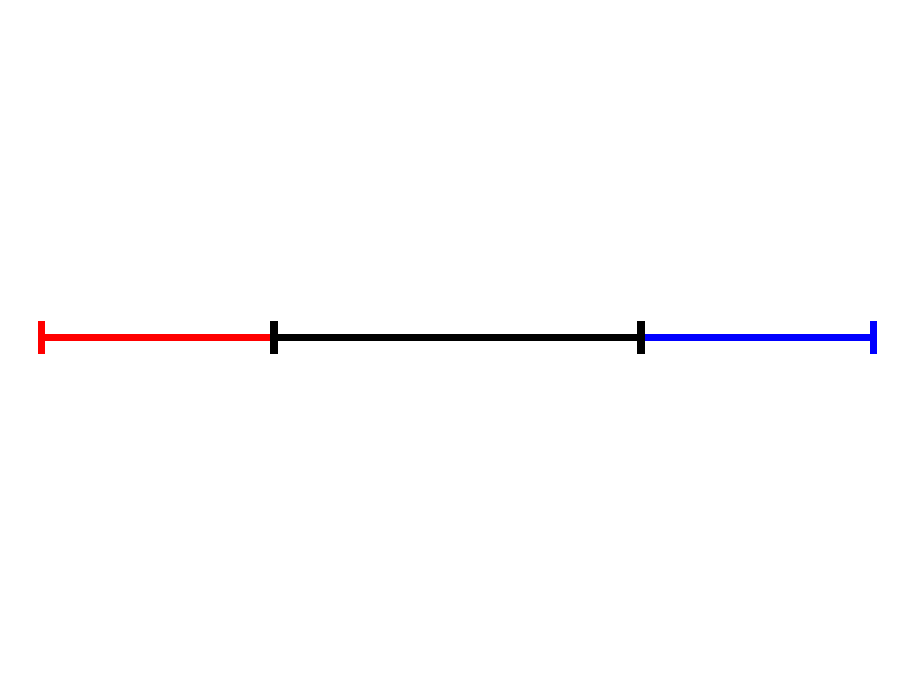
\includegraphics[scale=0.5,clip,trim=0 100 0 100]{figures/block1D.pdf}
		\end{tabular}
		&  
		\begin{tabular}{c}
			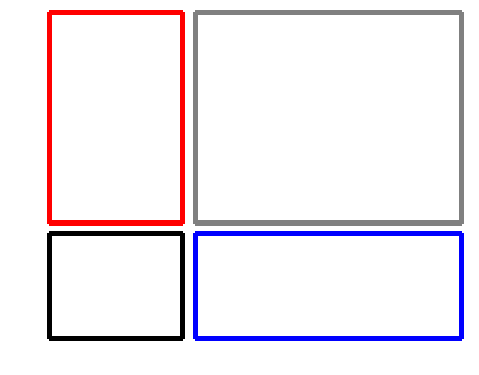
\includegraphics[scale=0.5]{figures/block2D.pdf}
		\end{tabular}
		
	\end{tabular}
	\caption{Example of a 1D (left) and 2D (right) multi-block domains}
	\label{fig:MB_domain}
\end{figure}

\begin{figure}[H]
	\centering
	\begin{tabular}{cc}
		\begin{tabular}{c}
			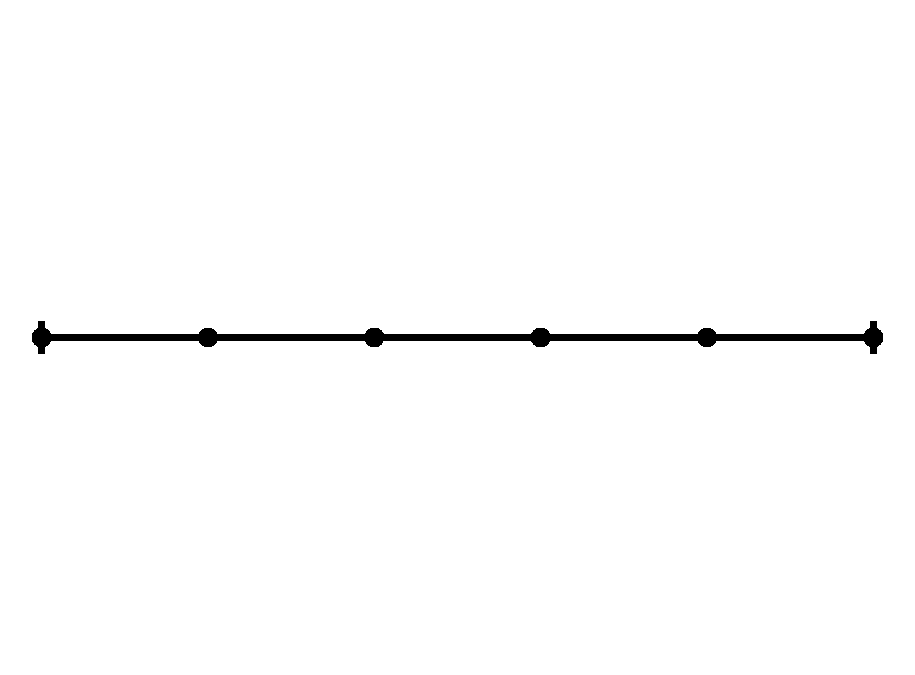
\includegraphics[scale=0.5, clip,trim=0 150 0 150]{figures/MBBL1D_eg1.pdf}
		\end{tabular}
		&
		\begin{tabular}{c}
			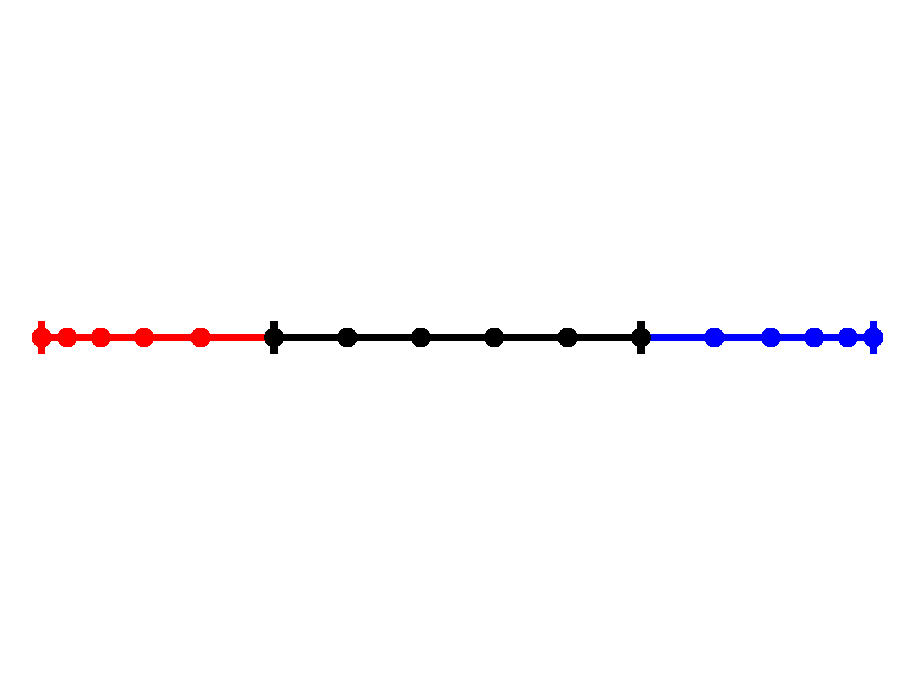
\includegraphics[scale=0.5, clip,trim=0 150 0 150]{figures/MBBL1D_eg2.pdf}
		\end{tabular}
	\end{tabular}
	\caption{Example of multi-block meshes -- 1-block uniform mesh (left) and 3-block mesh ordered as left-graded, uniform and right-graded blocks (right)}
	\label{fig:MBBL_1D_eg}
\end{figure}

\begin{figure}[H]
	\centering
	\begin{subfigure}[b]{0.45\textwidth}
		\centering
		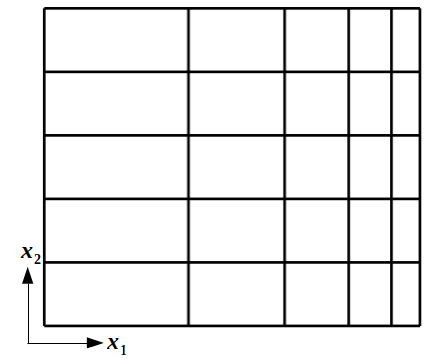
\includegraphics[scale=0.45]{figures/MBBL2D_eg1.png}
		\caption{\tiny\{rightBL\}$^{x_1}\,\,\otimes\,\,$\{uniform\}$^{x_2}$}
	\end{subfigure}
	\hspace{1cm}
	\begin{subfigure}[b]{0.45\textwidth}
		\centering
		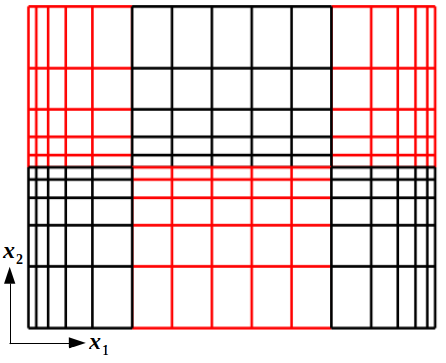
\includegraphics[scale=0.45]{figures/MBBL2D_eg2.png}
		\caption{\tiny\{leftBL, uniform, rightBL\}$^{x_1}\,\,\otimes\,\,$\{topBL, bottomBL\}$^{x_2}$}
	\end{subfigure}
	\caption{2D tensor-product MBBL meshes: one $(1\times1)$ block mesh  (left) and six $(3\times2)$ block mesh }
	\label{fig:MBBL_2D_eg}
\end{figure}

PUMImbbl mesh can be implemented in select non-convex domains in 2D by de-activating certain blocks. We will refer to these de-activated blocks as ``inactive-blocks" and the remaining blocks as ``active-blocks"

\begin{figure}[H]
	\centering
	\begin{subfigure}[b]{0.45\textwidth}
		\centering
		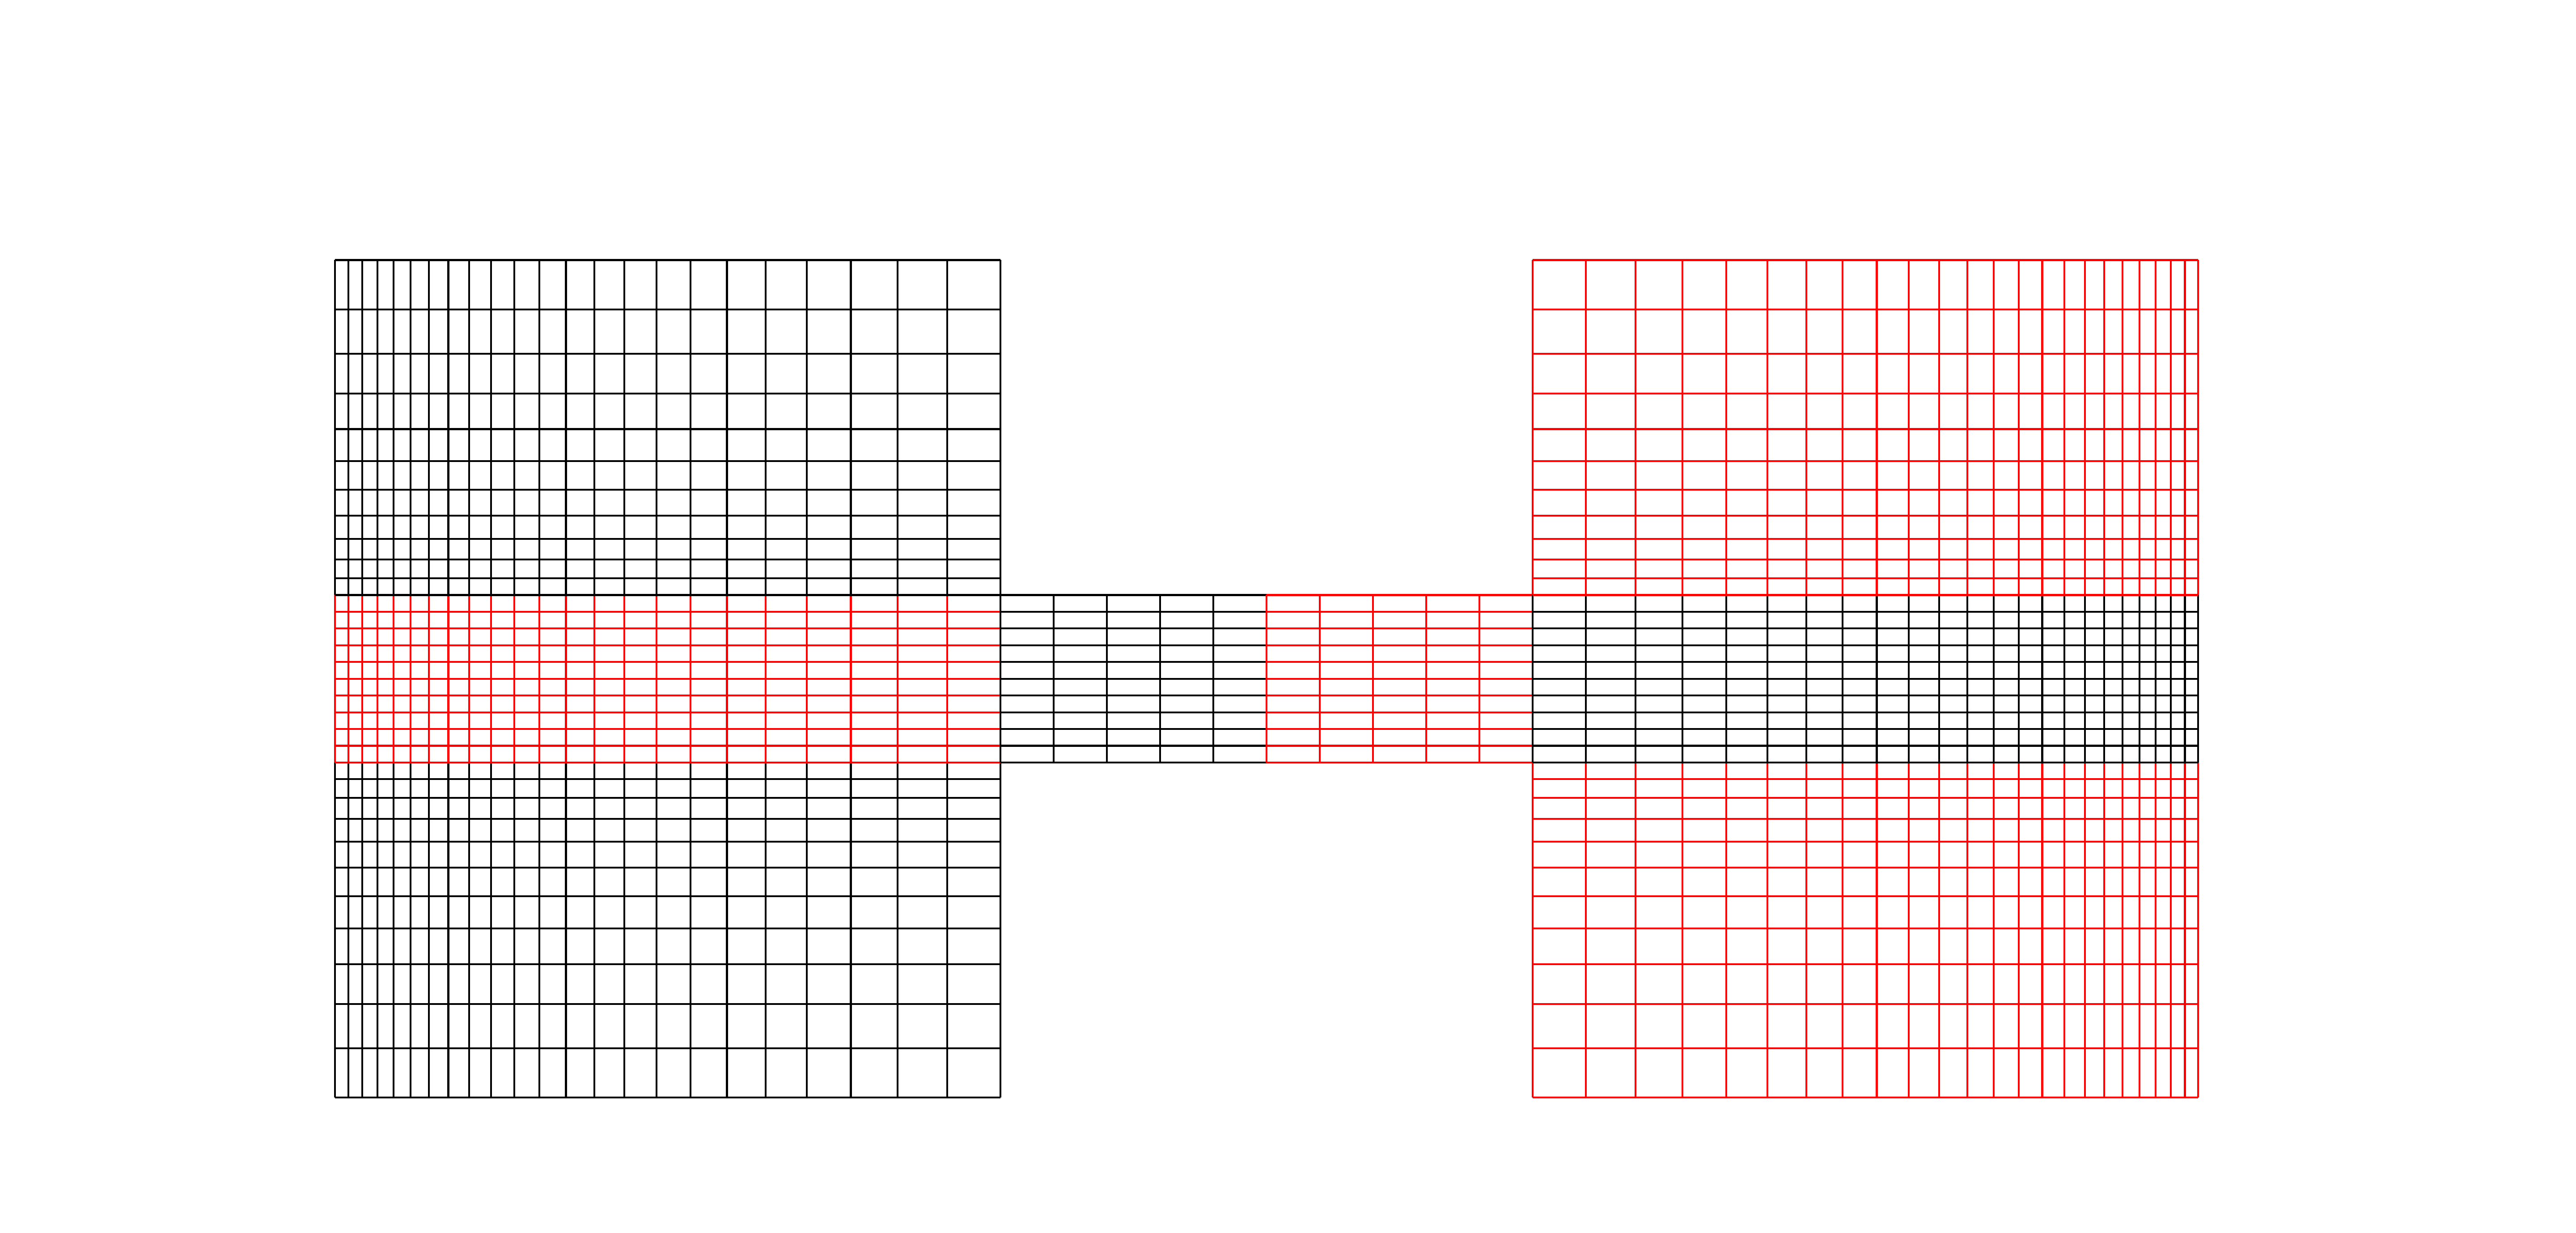
\includegraphics[scale=0.2,clip,trim=100 50 100 100]{figures/MBBL_nc_4x3.png}
		\caption{H-shaped domain}
	\end{subfigure}
	\hspace{0.25cm}
	\begin{subfigure}[b]{0.45\textwidth}
		\centering
		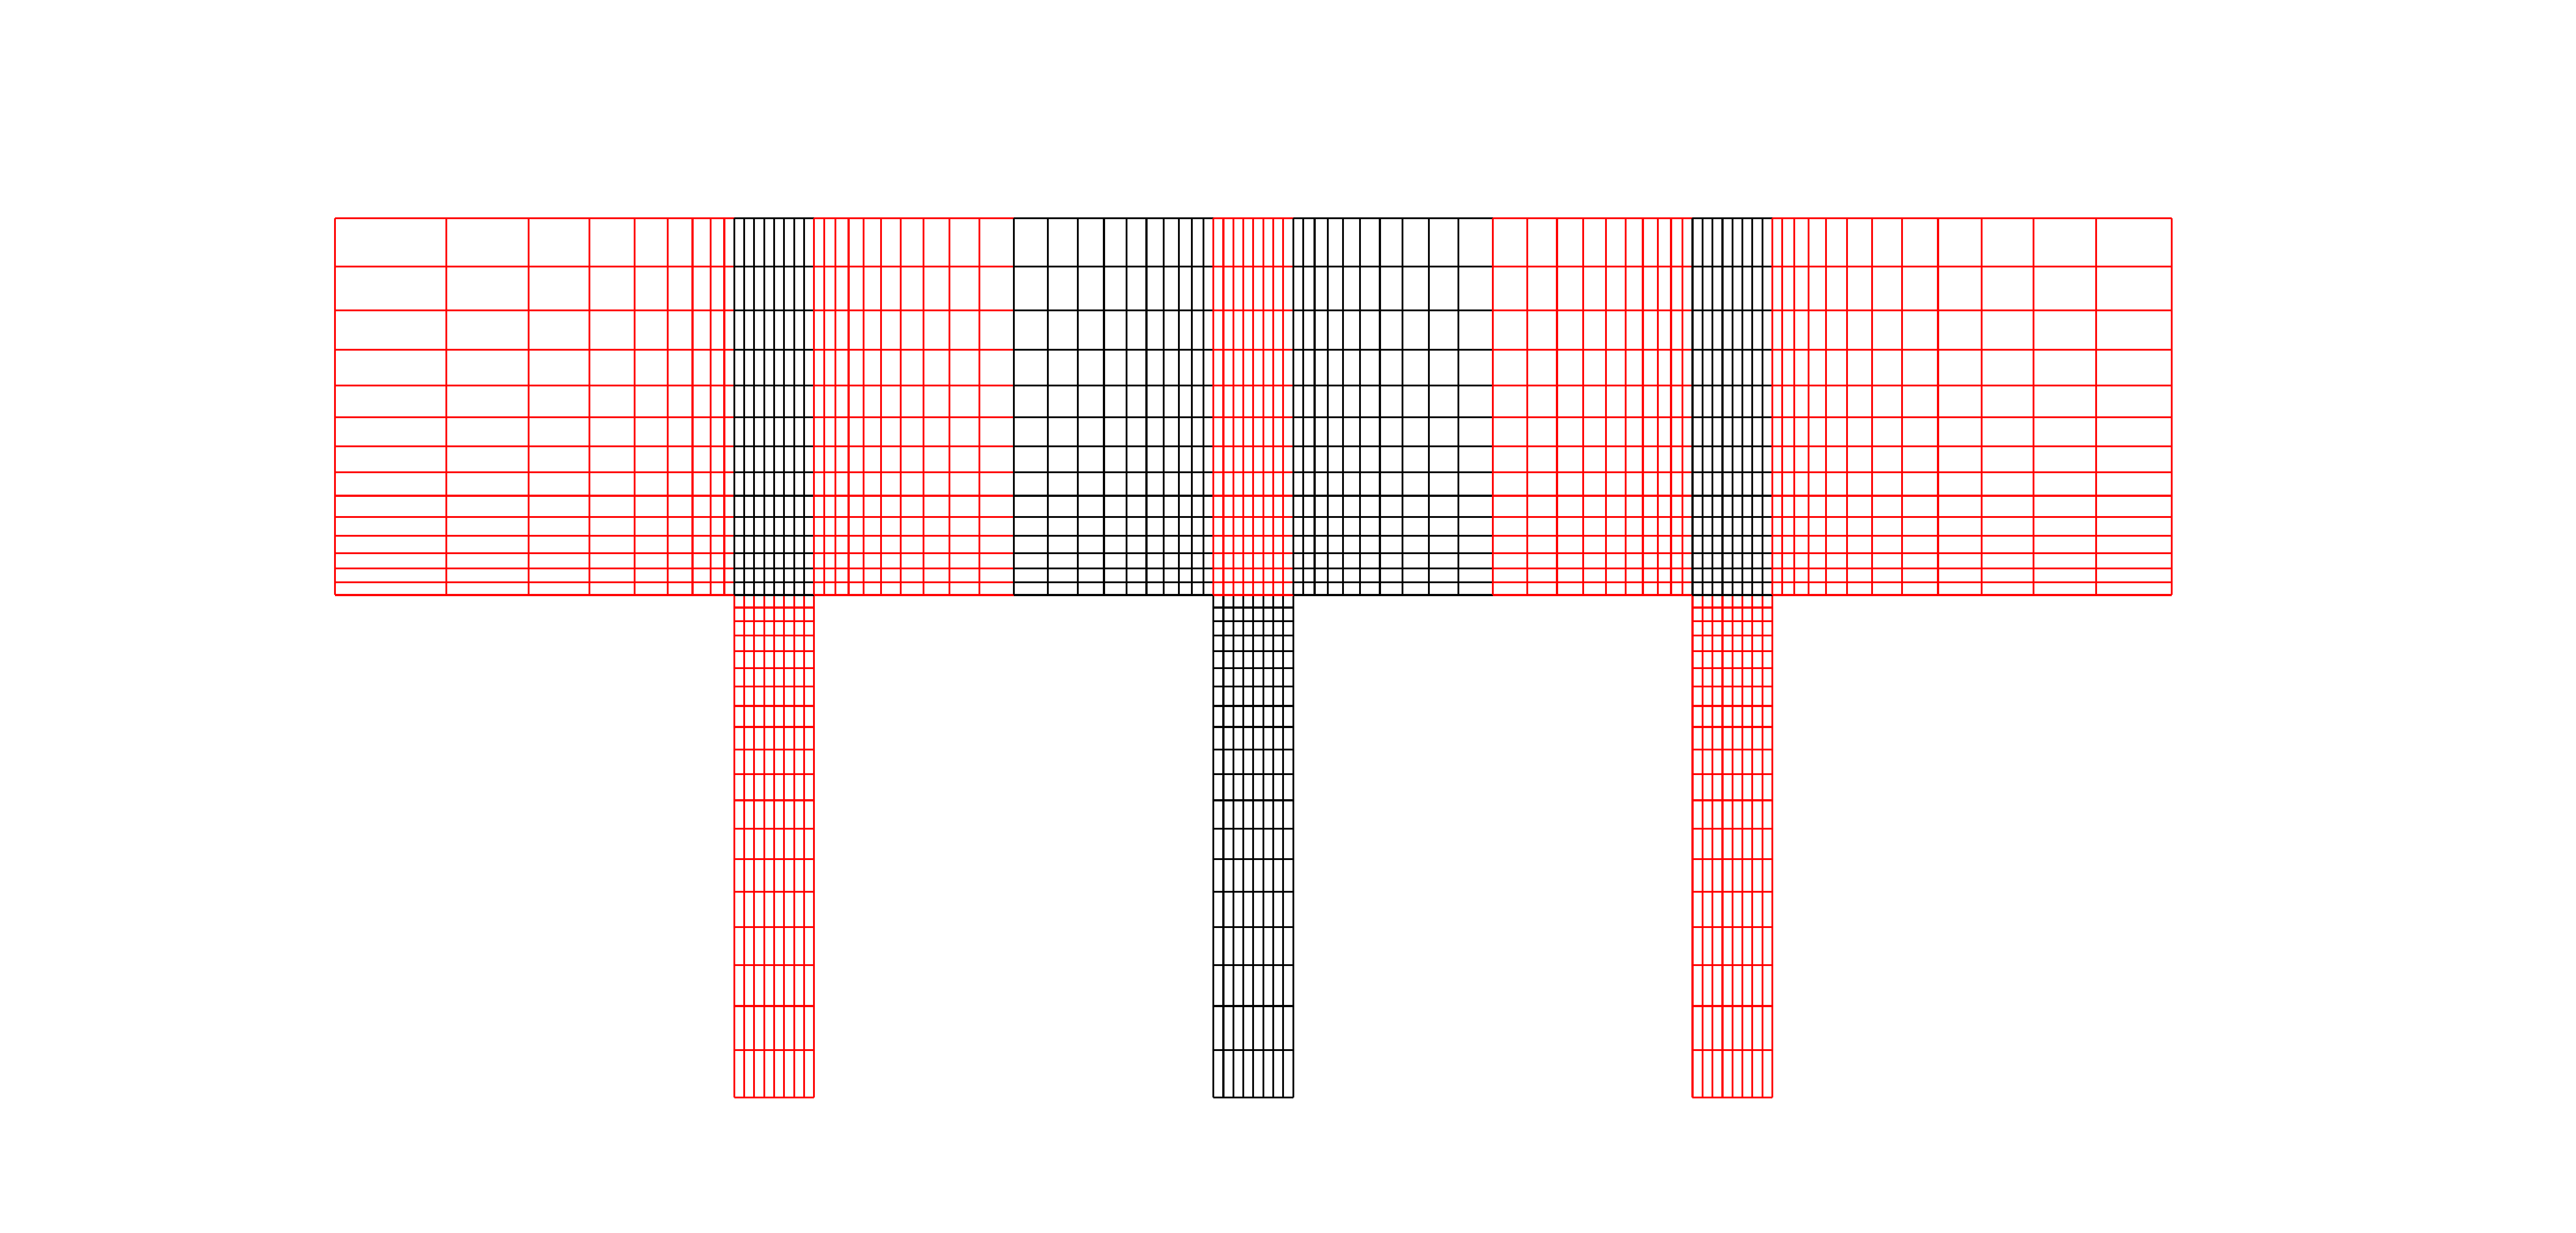
\includegraphics[scale=0.2,clip,trim=100 50 100 100]{figures/MBBL_nc_9x2.png}
		\caption{Tile-gap like domain}
	\end{subfigure}
	\caption{MBBL mesh with inactive blocks for non-convex domains}
	\label{fig:nonconvex_MBBL_2D_eg}
\end{figure} 

An advantage of the MBBL mesh is that it is not explicitly stored. Meshing inside each block is implicitly defined through a set of parameters. The parameterized multi-block mesh only need utmost 50 bytes of memory per block for the submesh parameters. All the other relevant mesh parameters needed for the PIC simulation can be calculated on-the-fly using the relations described above. 

\begin{table}[H]
	\centering
	\footnotesize
	\begin{tabular}{|l|l|l|}
		\hline
		Parameters         & Datatype              & Description                                                                                                        \\ \hline\hline
		$\xtil{N}$              & \texttt{int}          & Number of blocks in the domain                                                                                     \\ \hline
		$\xtil{n}^{el,total}$ & \texttt{int}          & \begin{tabular}[c]{@{}c@{}}Total number of elements in the domain \\(equal to sum of elements in each block)\end{tabular}                                    \\ \hline\hline
		$\xtil{x}^{min}_I$      & \texttt{double}       & Coordinate of the start of block $I$                                                                               \\ \hline
		$\xtil{x}^{max}_I$      & \texttt{double}       & Coordinate of the end of block $I$                                                                                 \\ \hline
		$meshtype_I$     & \texttt{unsigned int} & \begin{tabular}[c]{@{}c@{}}Total number of elements in the domain \\uniform (\texttt{0x01}), left-graded (\texttt{0x02}), right-graded (\texttt{0x04})\end{tabular}  \\ \hline
		$\xtil{n}^{el}_I$       & \texttt{int}          & Number of elements in block $I$                                                                                    \\ \hline
		$\xtil{t}_I$          & \texttt{double}       & \begin{tabular}[c]{@{}c@{}}Smallest element size in block $I$\\ (or regular element size in uniform blocks)   \end{tabular}                                                                             \\ \hline
		$\xtil{r}_I$            & \texttt{double}       & Geometric grading ratio of element sizes in block $I$                                                              \\ \hline
	\end{tabular}
	\caption{Parameterized multi-block boundary layer mesh}
	\label{tab:MBBL_params}
\end{table}

For non-uniform mesh blocks, for faster PIC operations the node coordinates are stored explicitly (this opens the possibility to use a completely irregular mesh not defined by any analytical formulae).

\subsection{Element/Node ID conventions}
\subsubsection{Submesh IDs}
A 2D submesh block is indexed by two integers \texttt{(isub, jsub)}

\begin{itemize}
	\item Original rectangular multi-block domain is padded with one layer of \textbf{ghost-blocks} all around. If original set of blocks is $N_{x_1}\times N_{x_2}$, padded domain contains $(N_{x_1}+2)\times (N_{x_2}+2)$
	\item Length of each padded ghost block layer is 1000 times actual domain length along the padded-direction
	\item This is done for algorithmic convenience, makes the original $N_{x_1}\times N_{x_2}$ blocks all interior blocks, which means homogeneous algorithm implementation with no need for special treatments for blocks in boundary
\end{itemize}
\begin{figure}[H]
	\centering
	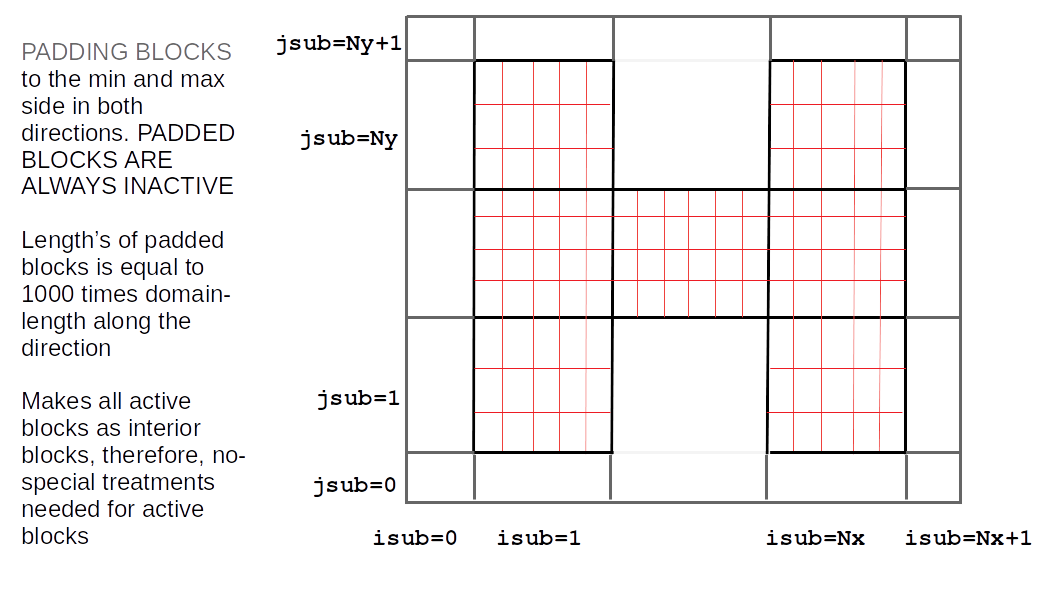
\includegraphics[trim=250 0 0 0,clip,scale=0.35]{figures/Block-Padding-2D.png}
	\caption{\texttt{isub} -- submesh ID in x1-direction}{\texttt{jsub} -- submesh ID in x2-direction}			
\end{figure}
\noindent Possible submesh ID values:
\begin{equation*}
1 \le \texttt{isub} \le N^{submesh}_{x_1} \qquad 1 \le \texttt{jsub} \le N^{submesh}_{x_2}
\end{equation*}
$N^{submesh}_{x_1},N^{submesh}_{x_2}$ -- Number of submesh blocks in x1, x2 directions respectively. Alternatively, the pairwise indices can also be flattened into one unique index and written as,\\
$\texttt{flattened\_sub\_ID} = \texttt{(jsub-1)} \times N^{submesh}_{x_1} + \texttt{(isub-1)}$

\subsubsection{Local Cell IDs}
A cell inside a submesh block is indexed by two integers \texttt{(icell, jcell)}
\begin{figure}[H]
	\centering
	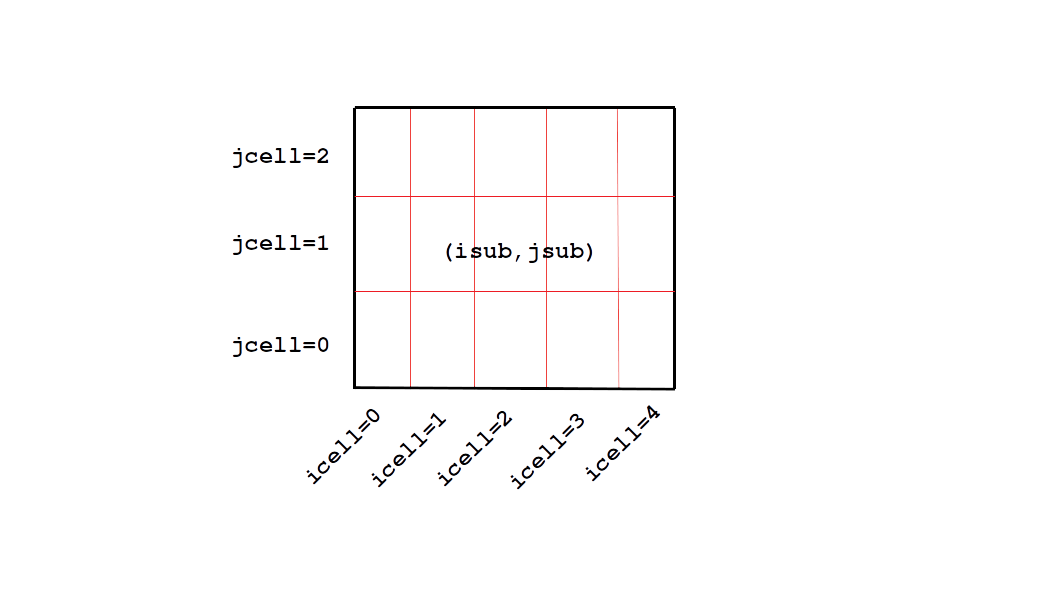
\includegraphics[trim=170 100 200 100,clip,scale=0.35]{figures/local_cell_ID.png}
	\caption{\texttt{icell} -- local cell ID in x1-direction}{\texttt{jcell} -- local cell ID in x2-direction}			
\end{figure}
\noindent Possible values:
\begin{equation*}
0 \le \texttt{icell} \le N^{el}_{x_1,\texttt{isub}}-1 \qquad 0 \le \texttt{jcell} \le N^{el}_{x_2,\texttt{jsub}}-1
\end{equation*}
$N^{el}_{x_1,\texttt{isub}}$ -- Number of elements along x1-direction in x1-block with ID \texttt{isub}\\
$N^{el}_{x_2,\texttt{jsub}}$ -- Number of elements along x2-direction in x2-block with ID \texttt{jsub}

Alternatively, the pairwise indices can also be flattened into one unique index and written as,\\
$\texttt{flattened\_cell\_ID} = \texttt{jcell} \times N^{el}_{x_1,\texttt{isub}} + \texttt{icell}$

\subsubsection{Component-wise Global Cell IDs}
Same as global row/column index of a cell in rectilinear mesh
\begin{figure}[H]
	\centering
	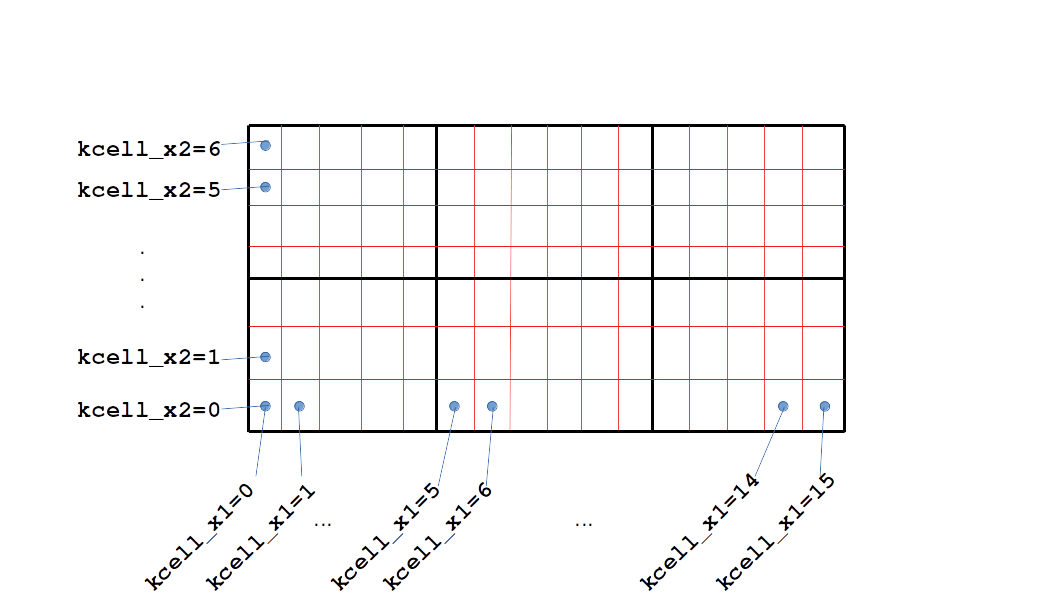
\includegraphics[trim=50 0 200 120,clip,scale=0.3]{figures/global_1D_cell_ID.png}
	\caption{\texttt{kcell\_x1} -- component-wise global cell ID in x1-direction}{\texttt{kcell\_x2} -- component-wise global cell ID in x2-direction}			
\end{figure}
\noindent Possible values:
\begin{equation*}
0 \le \texttt{kcell\_x1} \le N^{el,tot}_{x_1}-1 \qquad 0 \le \texttt{kcell\_x2} \le N^{el,tot}_{x_2}-1
\end{equation*}
$N^{el,tot}_{x_1},N^{el,tot}_{x_2}$ -- Number of total elements along x1, x2 directions respectively

\subsubsection{Component-wise Global Node IDs}
\begin{figure}[H]
	\centering
	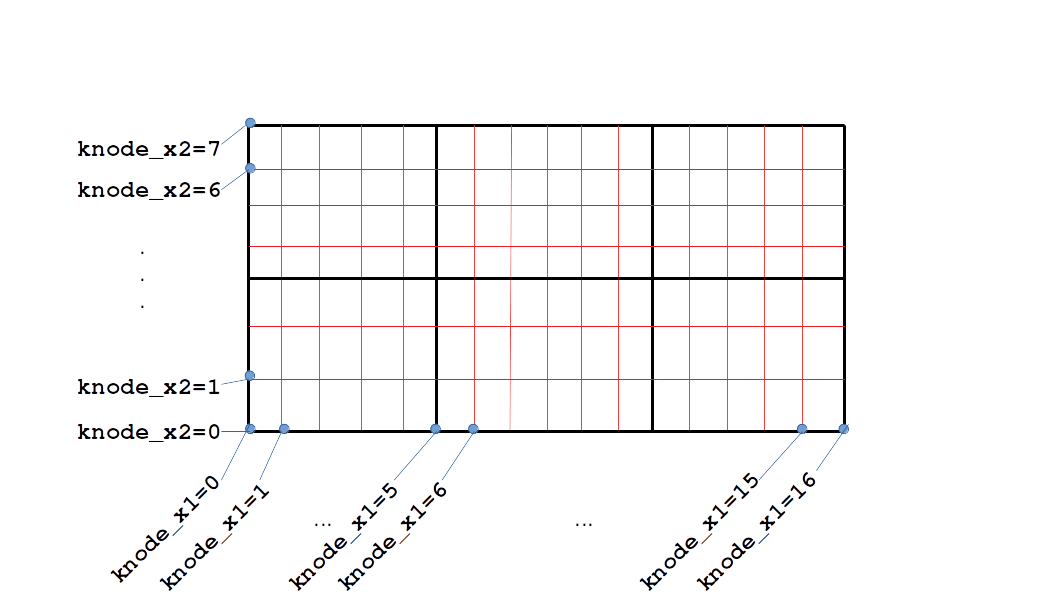
\includegraphics[trim=50 0 200 100,clip,scale=0.35]{figures/global_1D_node_ID.png}
	\caption{\texttt{knode\_x1} -- component-wise global cell ID in x1-direction}{\texttt{knode\_x2} -- component-wise global cell ID in x2-direction}			
\end{figure}
\noindent Possible values:
\begin{equation*}
0 \le \texttt{knode\_x1} \le N^{el,tot}_{x_1} \qquad 0 \le \texttt{knode\_x2} \le N^{el,tot}_{x_2}
\end{equation*}

\subsection{2D Global Element and Node conventions}
\subsubsection{Full Mesh (No Inactive Blocks)}
\textbf{2D Element Numbering:}  For a mesh with no inactive blocks the figure below show how the elements are numbered
\begin{figure}[H]
	\centering
	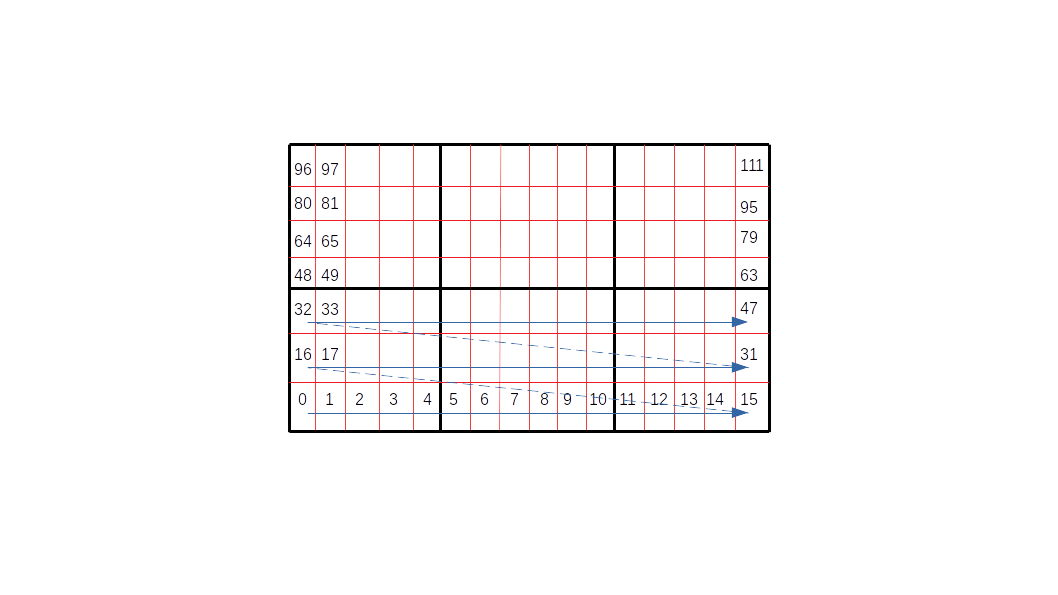
\includegraphics[trim=140 100 200 100,clip,scale=0.35]{figures/FullMesh_ElemNumbered.png}
	\caption{$N^{submesh}_{x_1}=3$,$N_{x_1}^{el,tot}=16$        $N^{submesh}_{x_2}=2$,$N_{x_2}^{el,tot}=7$}			
\end{figure}
The global cell ID in 2D space \texttt{global\_2D\_cell} is computed from component-wise global cell IDs (\texttt{kcell\_x1}, \texttt{kcell\_x2}) i.e. global row and column IDs as
\begin{figure}[H]
	\centering
	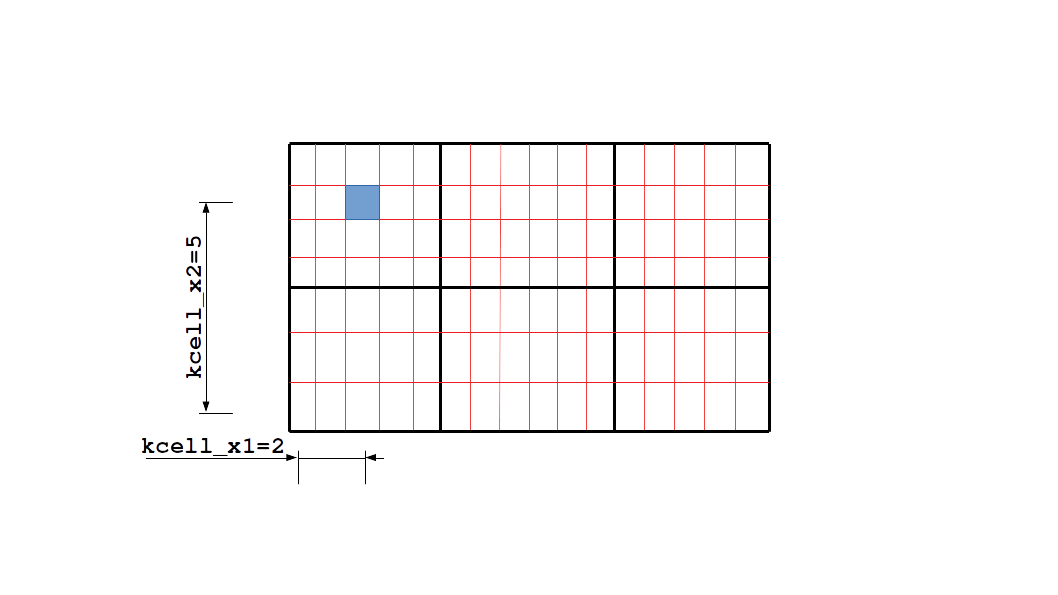
\includegraphics[trim=140 100 200  100,clip,scale=0.35]{figures/FullMesh_ElemIDCalc.png}
	\caption{$\texttt{global\_2D\_cell} = \texttt{kcell\_x2}\times N_{x_1}^{el,tot}+\texttt{kcell\_x1} = 5(16)+2 = 82$}			
\end{figure}

\noindent Possible values:
\begin{equation*}
0 \le \texttt{global\_2D\_cell} \le N^{el,tot}_{2D}-1
\end{equation*}
$N^{el,tot}_{2D}$ -- Total number of elements in the 2D domain.\\ On a full mesh $N^{el,tot}_{2D} = N^{el,tot}_{x_1}\times N^{el,tot}_{x_2}$

\vspace*{1cm}

\noindent\textbf{2D Node Numbering:} For a mesh with no inactive blocks the figure below show how the nodes are numbered 

\begin{figure}[H]
	\centering
	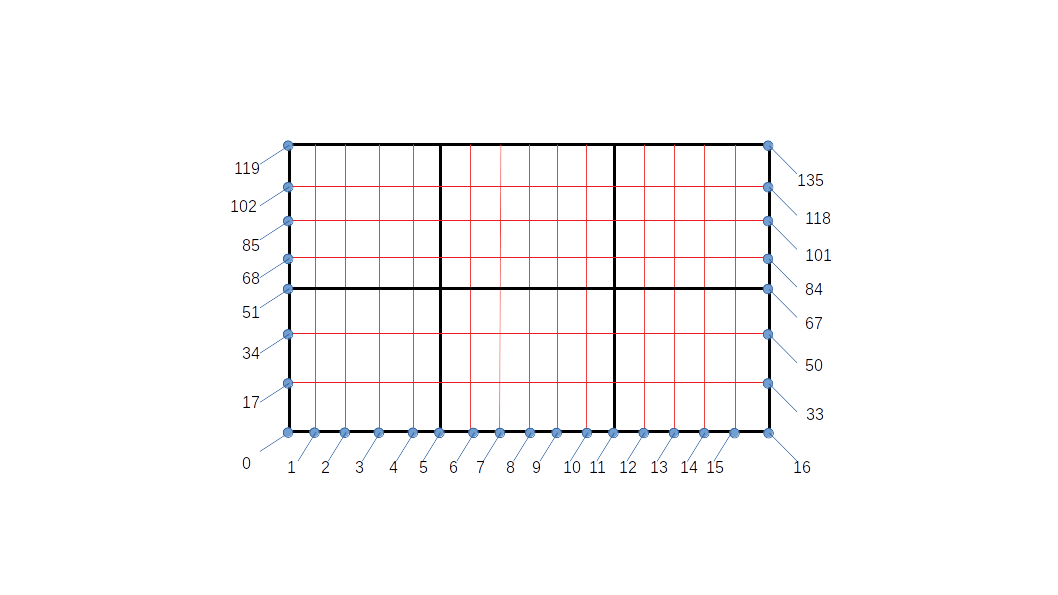
\includegraphics[trim=180 50 200 100,clip,scale=0.35]{figures/FullMeshNodeNumbered.png}
	\caption{Node numbering is done similar to element numbering}
\end{figure}

\begin{figure}[H]
	\centering
	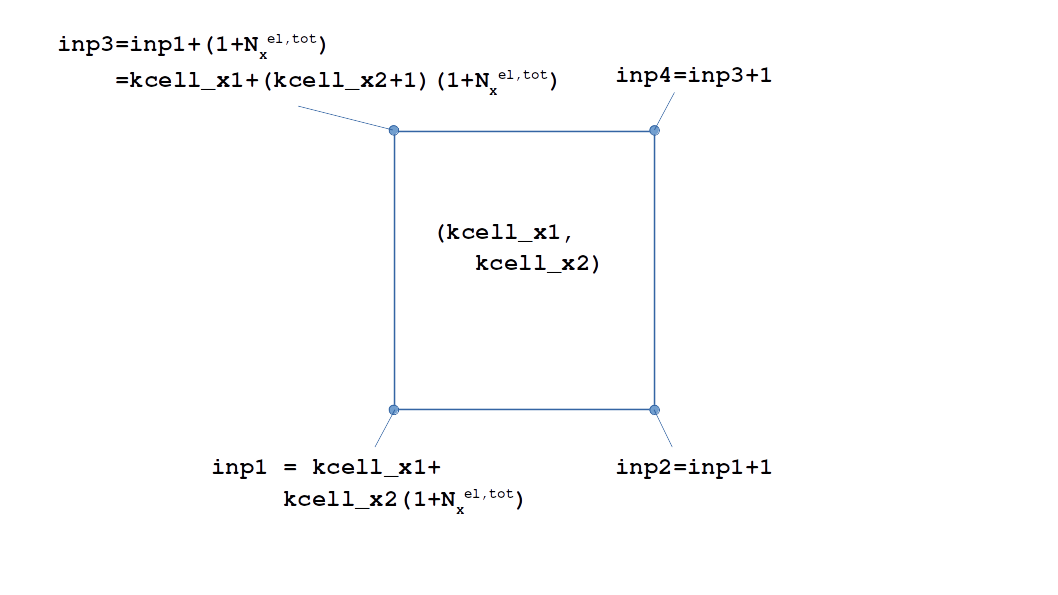
\includegraphics[scale=0.3]{figures/FullMeshNodeIDCalc.png}
	\caption{Global Node IDs associated with a given element can be calculated from global column index \texttt{kcell\_x1}, global row index \texttt{kcell\_x2} and total elements along x1-direction $N_{x_1}^{el,tot}$}			
\end{figure}

It's only essential to compute the node IDs of left-bottom \texttt{(inp1)} and left-top \texttt{(inp3)} nodes. Their right counterparts \texttt{(inp2 and inp4)} can be obtained by incrementing the values by 1. 

\noindent Possible values:
\begin{equation*}
0 \le \texttt{inp} \le N^{np,tot}_{2D}-1
\end{equation*}
$N^{np,tot}_{2D}$ -- Total number of nodes in the 2D domain.\\ On a full mesh $N^{np,tot}_{2D} = \left(N^{el,tot}_{x_1}+1\right)\times \left(N^{el,tot}_{x_2}+1\right)$

\subsubsection{Mesh with Inactive Blocks}
\textbf{2D Element Numbering:}  For a mesh with inactive blocks the figure below show how the elements are numbered
\begin{figure}[H]
	\centering
	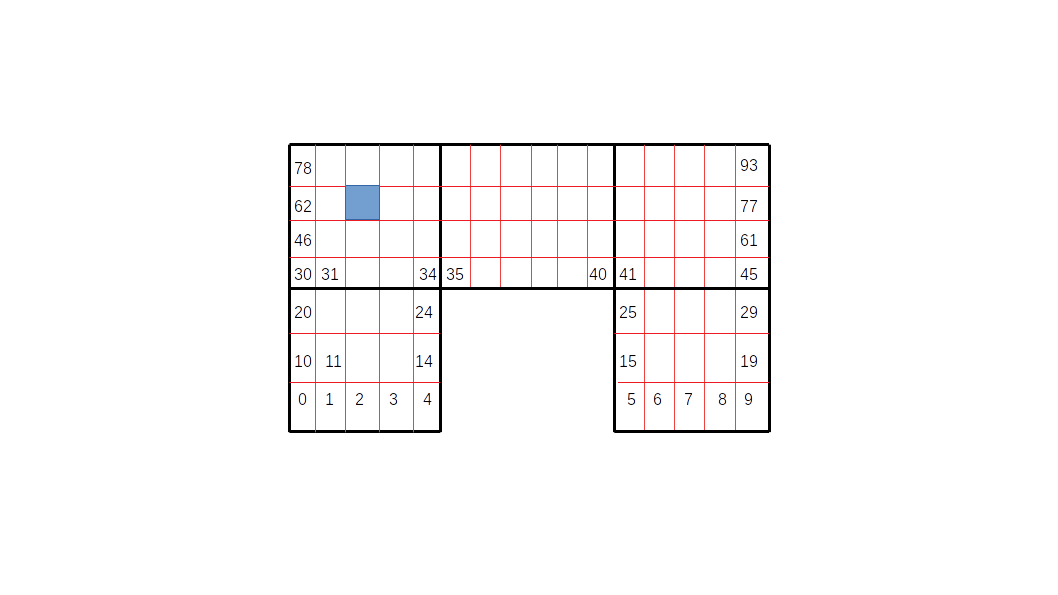
\includegraphics[trim=140 100 200 100,clip,scale=0.35]{figures/InactiveMesh_ElemNumbered.png}		
\end{figure}
Elements in the inactive blocks are skipped while numbering. For the sake of analytical computation of node IDs it is necessary to keep track of how many elements are skipped for for each row in each x1-block (see figure below)  
\begin{figure}[H]
	\centering
	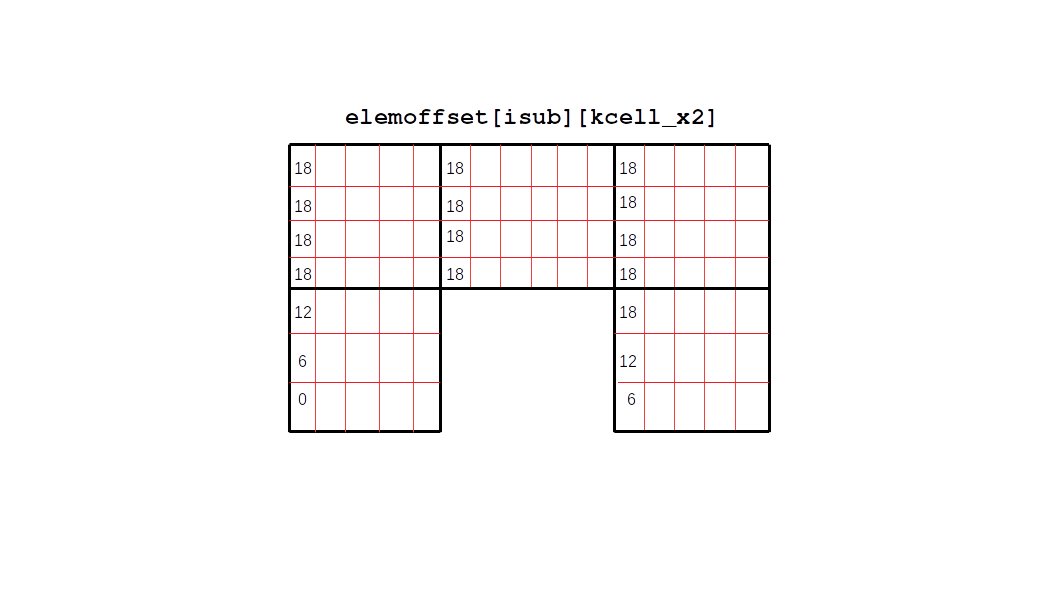
\includegraphics[trim=140 100 200 100,clip,scale=0.35]{figures/ElemOffset.png}		
\end{figure}

\paragraph{Element ID calculation -- Example}
The global element ID can be computed using the same expression used in full mesh and subtracting an offset (which tracks the number of skipped elements)
\begin{figure}[H]
	\centering
	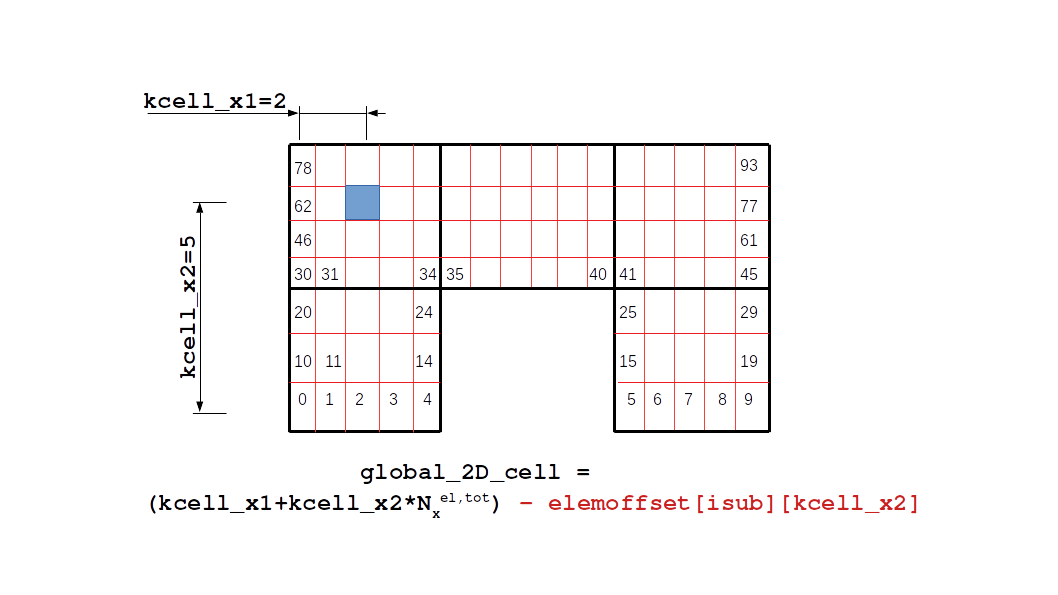
\includegraphics[trim=140 20 140 80,clip,scale=0.35]{figures/InactiveMesh_ElemIDCalc.png}
	\caption{\texttt{global\_2D\_cell = 2+5$\times$16-18 = 64}}			
\end{figure}

\noindent\textbf{Computation of \texttt{elemoffset} without explicit storage}
The value of offset for each row in a x1-submesh block can be obtained by storing two additional integers for every submesh block
\begin{figure}[H]
	\centering
	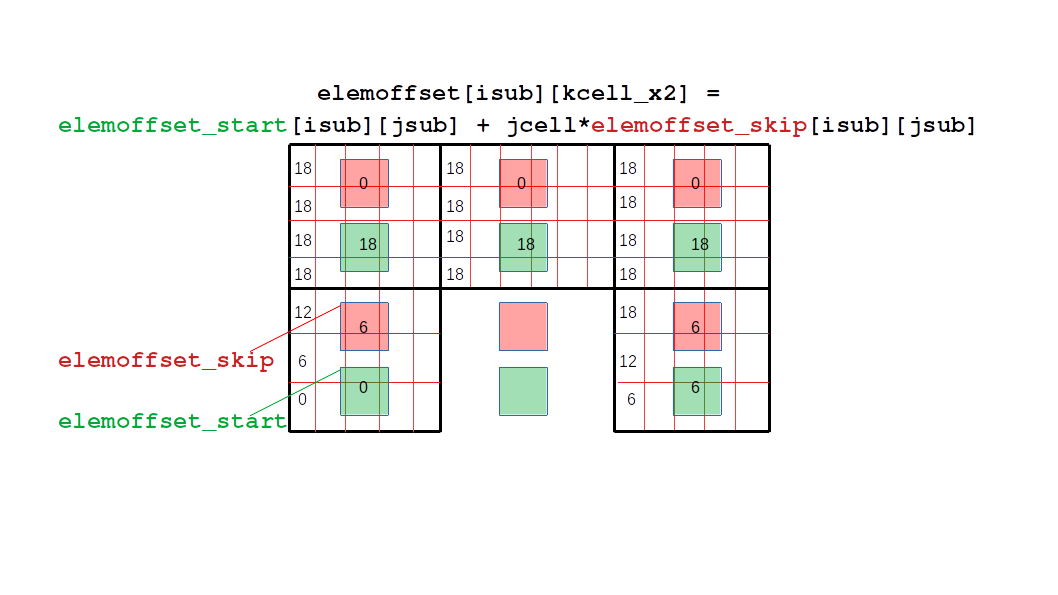
\includegraphics[trim=50 100 80 80,clip,scale=0.35]{figures/ElemOffsetCalc.png}		
\end{figure}

\noindent\textbf{2D Node Numbering:} For a mesh with inactive blocks the figure below show how the nodes are numbered
\begin{figure}[H]
	\centering
	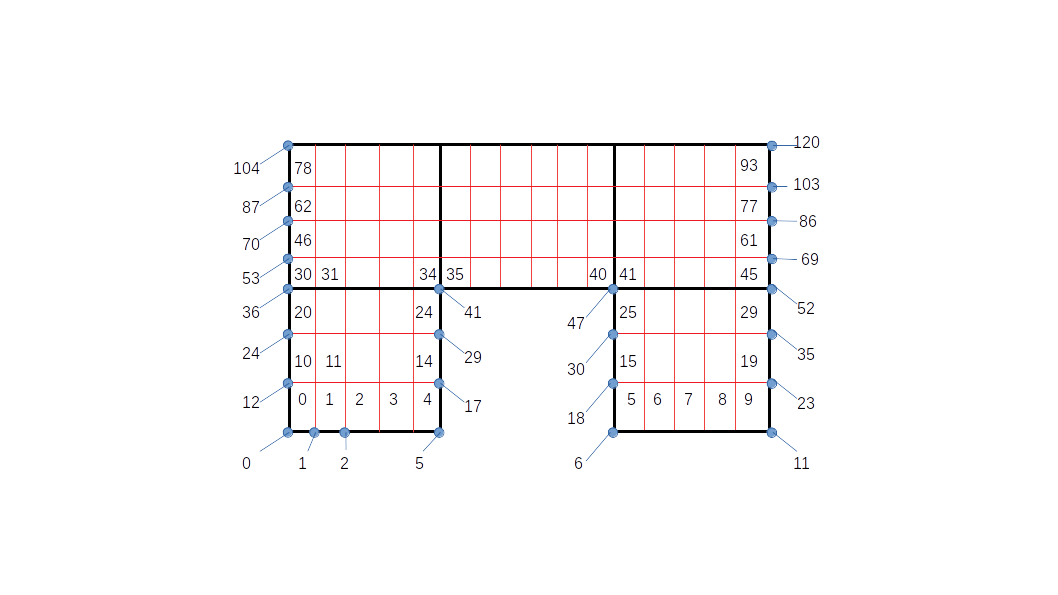
\includegraphics[trim=140 100 200 100,clip,scale=0.35]{figures/InactiveMesh_NodeNumbered.png}		
\end{figure} 

\begin{figure}[H]
	\centering
	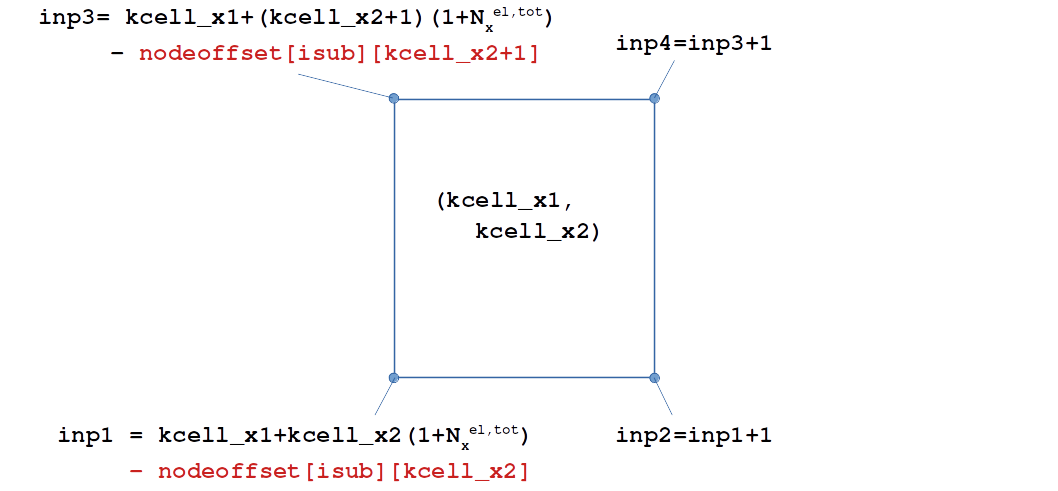
\includegraphics[scale=0.35]{figures/InactiveMeshNodeIDCalc.png}	
\end{figure}

Same as element numbering, we skip the nodes in the inactive blocks while numbering. However, the offset that keeps track of skipped nodes DO NOT follow the same `nice' pattern inside a submesh block as the element offsets. 
\begin{figure}[H]
	\centering
	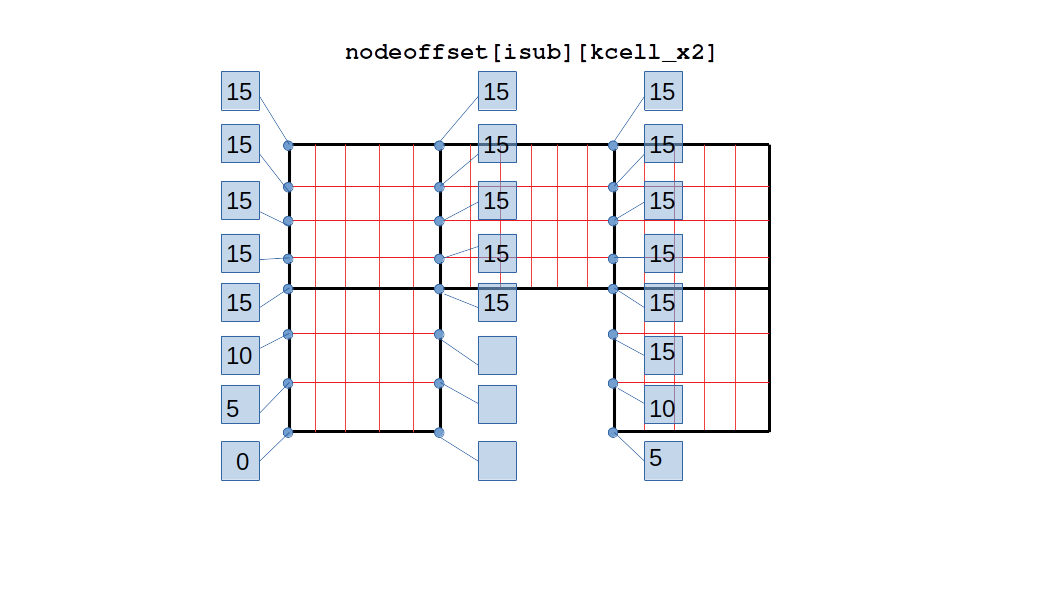
\includegraphics[trim=140 100 200 25,clip,scale=0.3]{figures/NodeOffset.png}\\	
	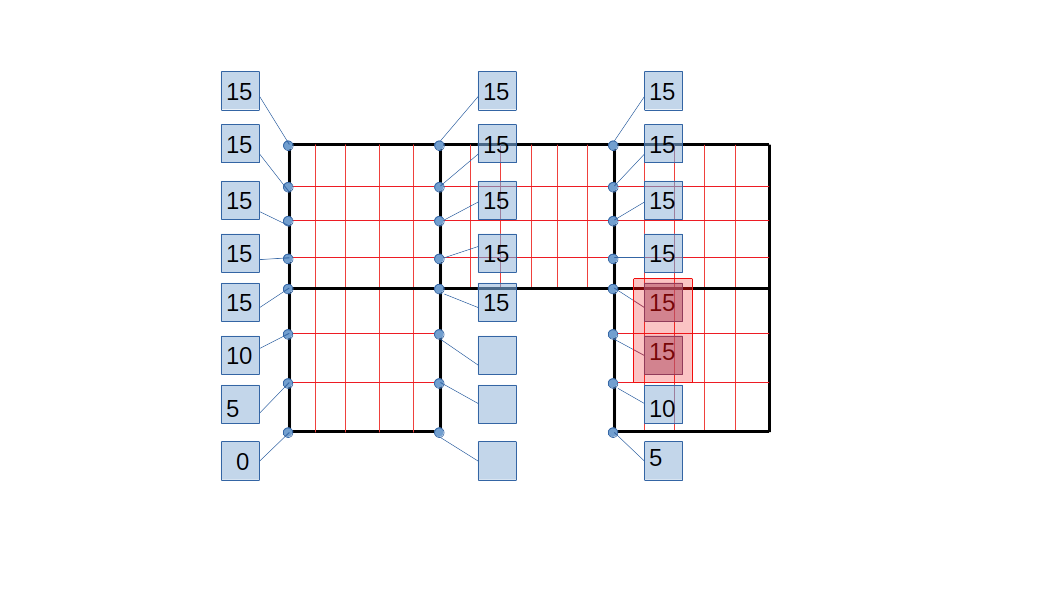
\includegraphics[trim=140 100 200 25,clip,scale=0.3]{figures/NodeOffset_Exception-1.png}
	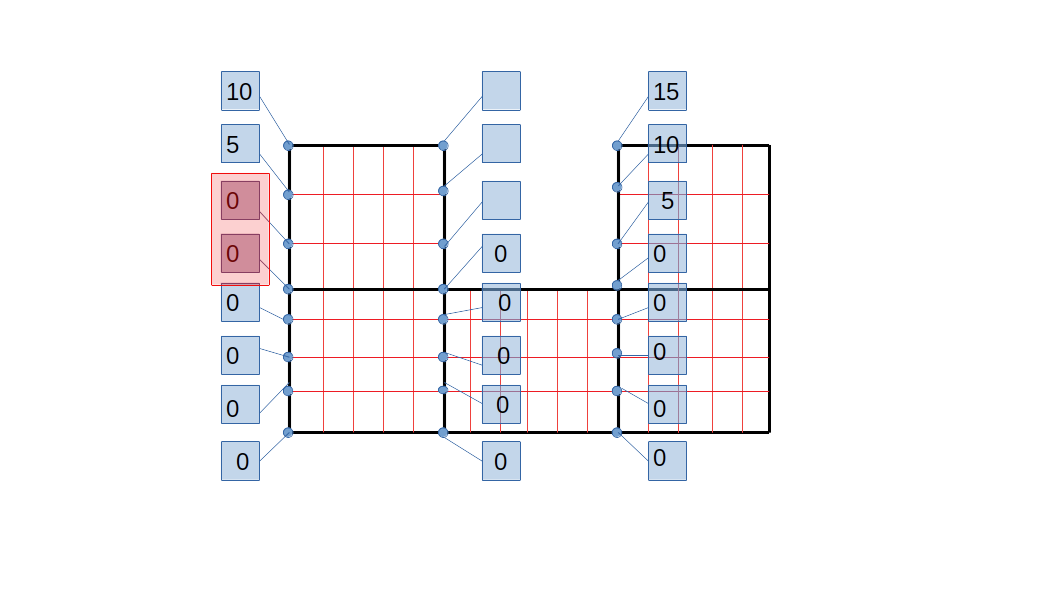
\includegraphics[trim=140 100 200 25,clip,scale=0.3]{figures/NodeOffset_Exception-2.png}
	\caption{Examples where \texttt{nodeoffset} do not follow the same pattern as the rest of the block}	
\end{figure}

Similar to the variable \texttt{elemoffset\_skip}, for computation of number of skipped nodes three variables are needed -- \texttt{nodeoffset\_skip\_bot} (for bottom row of nodes in block), \texttt{nodeoffset\_skip\_mid} (for all rows in the block excluding the top-most and bottom-most rows), and \texttt{nodeoffset\_skip\_top} (for top row of nodes).
\begin{figure}[H]
	\centering
	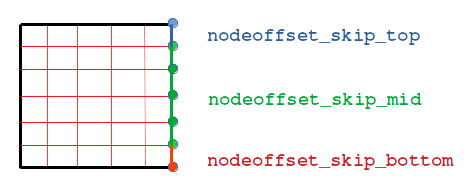
\includegraphics[scale=0.6]{figures/NodeOffset-new.png}	
\end{figure}

\paragraph{Node ID calculation -- Examples} The global node IDs will be computed similar to element IDs by subtracting the offset. The offset itself will be computed using the auxiliary variables \texttt{nodeoffset\_start}, \texttt{nodeoffset\_skip\_bot}, \texttt{nodeoffset\_skip\_mid} and \texttt{nodeoffset\_skip\_top}.

\begin{figure}[H]
	\centering
	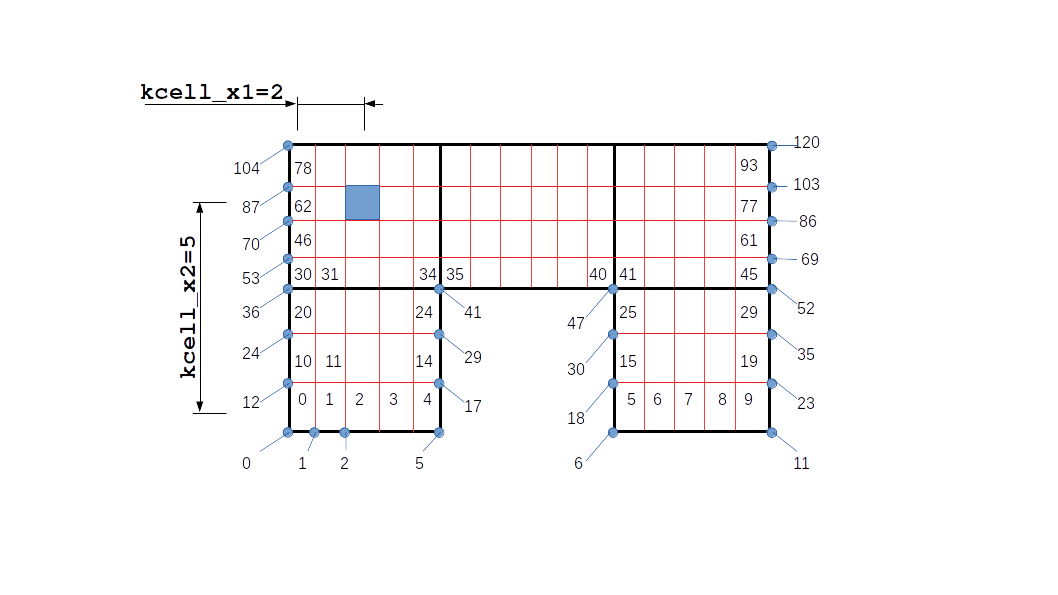
\includegraphics[trim=140 120 200 75,clip,scale=0.4]{figures/InactiveMeshNodeIDCalc-Eg1.png}	
	\caption{\texttt{inp1=2+5$\times$17-15=72}}{\texttt{inp3=2+6$\times$17-15=89}}
\end{figure}

\begin{figure}[H]
	\centering
	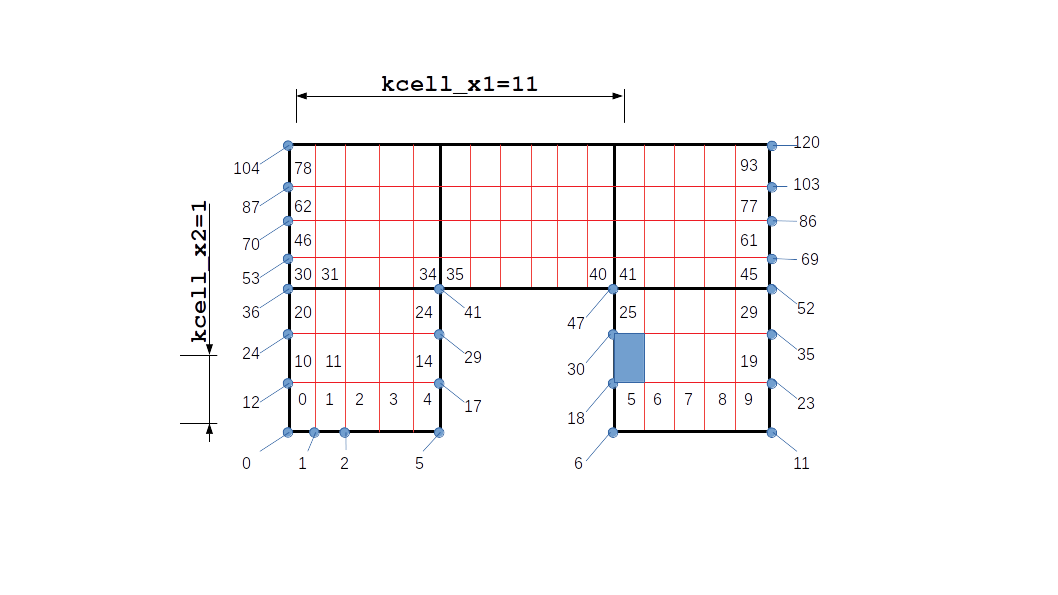
\includegraphics[trim=140 120 200 75,clip,scale=0.4]{figures/InactiveMeshNodeIDCalc-Eg2.png}	
	\caption{\texttt{inp1=11+1$\times$17-10=18}}{\texttt{inp3=11+2$\times$17-15=30}}
\end{figure}

\subsubsection{Block Entity Classification}
Every submesh block in a 2D mesh is characterized by 4 edges and 4 vertices
\begin{figure}[H]
	\centering
	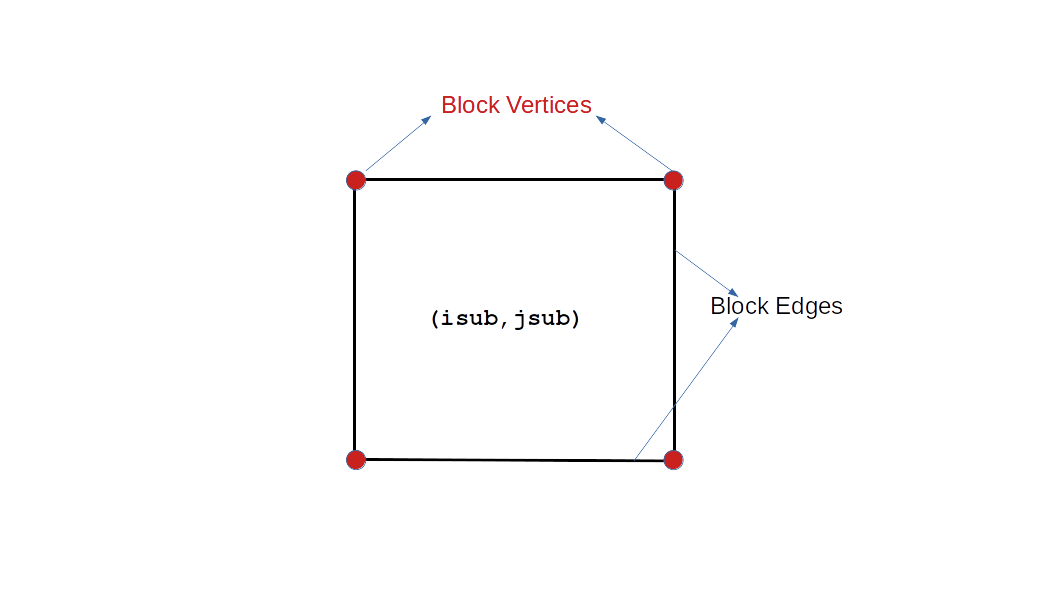
\includegraphics[trim=140 120 200 75,clip,scale=0.35]{figures/Block-Classification.png}
\end{figure}
A vertex is a \textit{zero-dimensional entity} while the edge is an \textit{one-dimensional entity}. In order to apply different boundary/interface conditions at different locations, we need to ID these entities. In the following sections the convention used for edge and vertex numbering is explained. The convention is standard i.e. regardless of the activity of blocks in the mesh the convention holds. 
\paragraph{Standard Block-Edge Numbering}
The standardized ID-ing helps us come up with expressions to obtain the edge IDs of any given block as shown below
\begin{figure}[H]
	\centering
	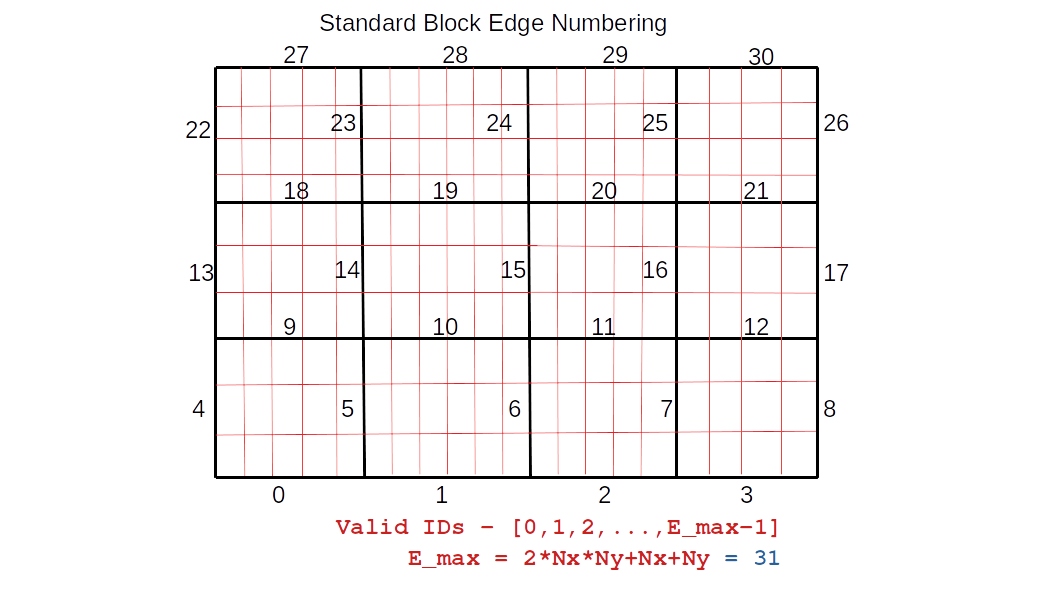
\includegraphics[trim=140 25 200 38,clip,scale=0.3]{figures/Block-Edge-Numbered.png}
	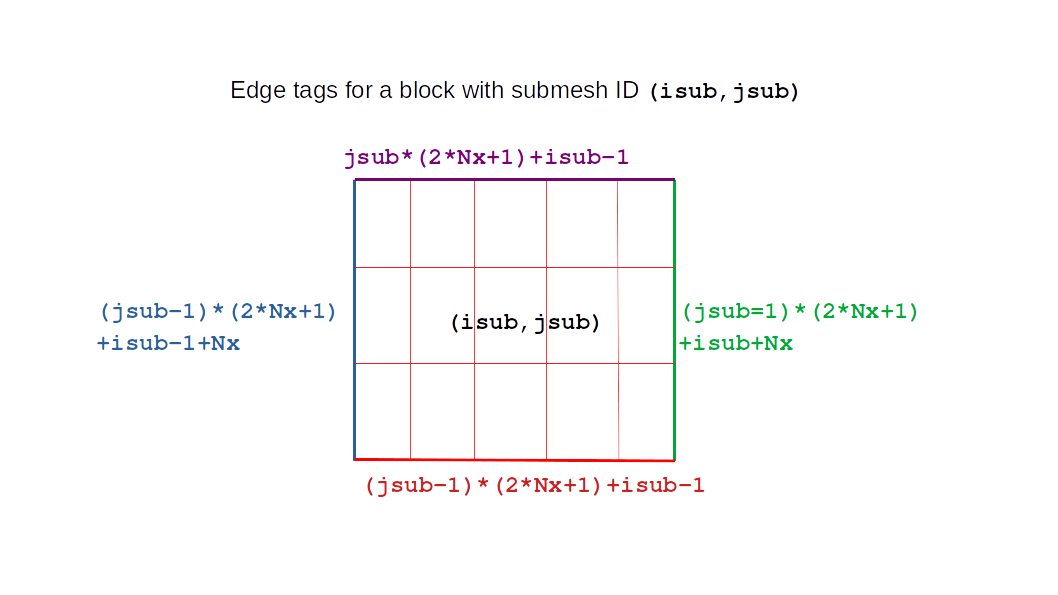
\includegraphics[trim=80 0 100 0,clip,scale=0.3]{figures/Std-Block-Edge-IDs.png}
\end{figure}


\paragraph{Standard Block-Vertex Numbering}
Similarly, we follow similar standardized numbering for block vertcices. Any given block the vertex IDs can be expressed as shown below
\begin{figure}[H]
	\centering
	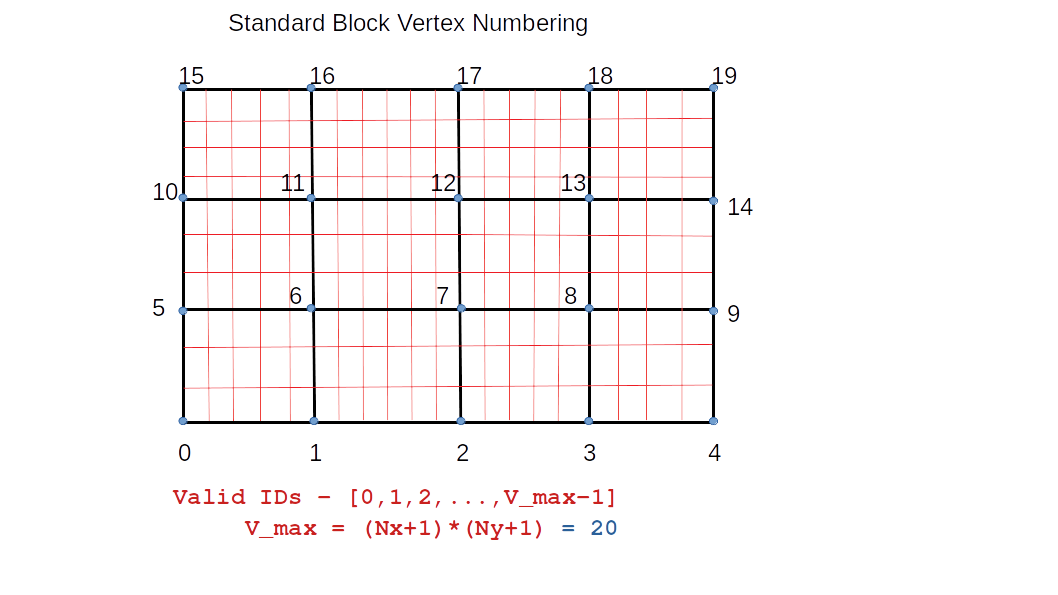
\includegraphics[trim=140 40 200 38,clip,scale=0.3]{figures/Block-Vert-Numbered.png}
	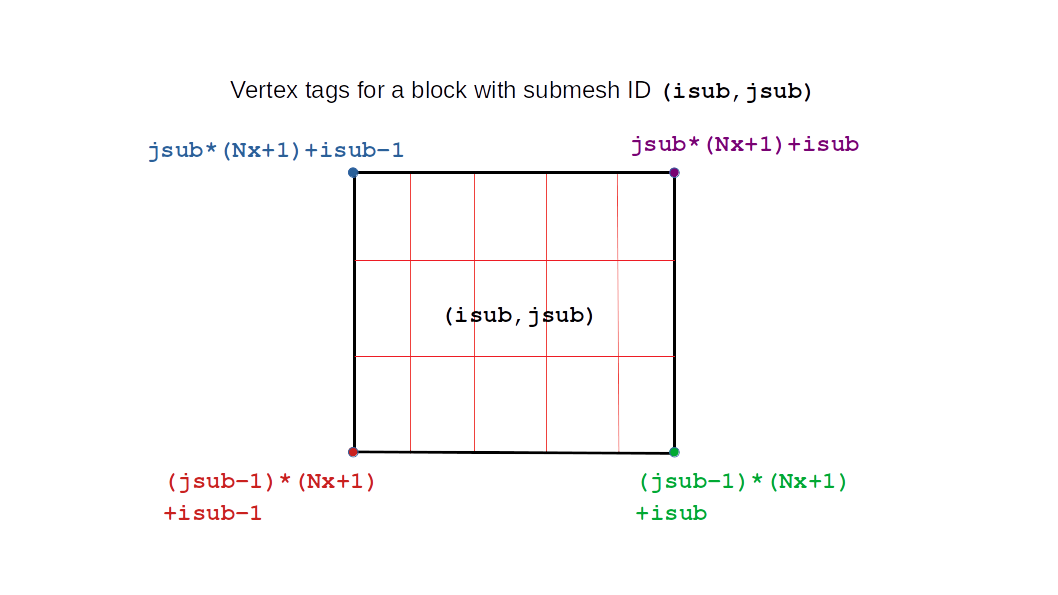
\includegraphics[trim=140 0 100 0,clip,scale=0.3]{figures/Std-Block-Vert-IDs.png}
\end{figure}

For a mesh with inactive blocks, the scheme remains unchanged i.e. the tags corresponding entities in non-active blocks will be invalid
\begin{figure}[H]
	\centering
	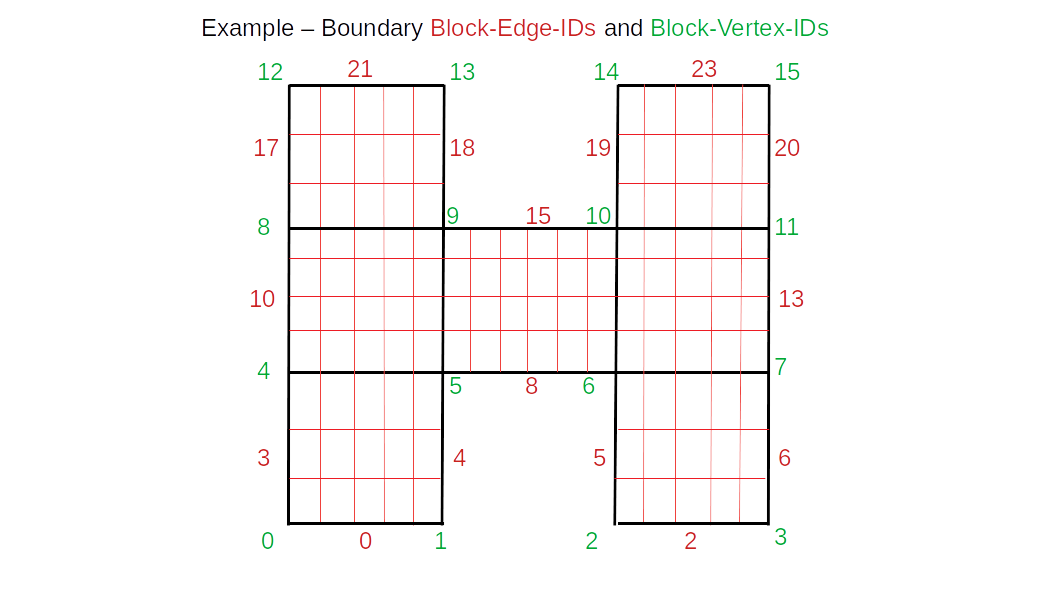
\includegraphics[trim=140 0 200 0,clip,scale=0.3]{figures/Block-EV-ID-Eg.png}
\end{figure}

\subsubsection{Boundary Edge/Vertex Information}
It is necessary to store some domain information on each of the classified block entities. These include -- 
\begin{itemize}
	\item Is an entity lie outside the domain boundary?
	\item Is an entity lie on the domain boundary?
	\item What is the direction of boundary normal for each boundary entity? 
\end{itemize} 

While these information can be obtained by checking the block activity status of relevant blocks associated with the boundary, for faster access of such information, it is necessary to store such data. For example, the boundary normal direction at locations of boundary vertices and edges can provide insights to how mesh-level operations like gradient computation can be carried out at those places.   

%A boolean value for each edge/vertex stores if the given entity falls on the domain boundary or not. The library provides the API \texttt{where\_is\_node()} which takes the component-wise node IDs (\texttt{knode\_x1}, \texttt{knode\_x2}) and returns necessary information on the node such as if node is active, if node is on boundary, if a boundary node is on block-edge or block-vertex. Refer to later sections for API usage. Aside from boundary classification of block edges/vertices, the boundary normal directions are also stored on all boundary entities.   

\begin{figure}[H]
	\centering
	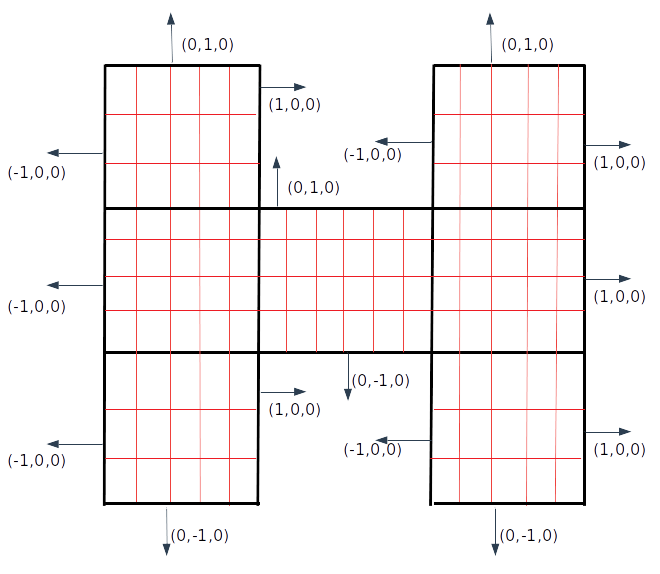
\includegraphics[scale=0.33]{figures/EdgeBdryNrml.png}
	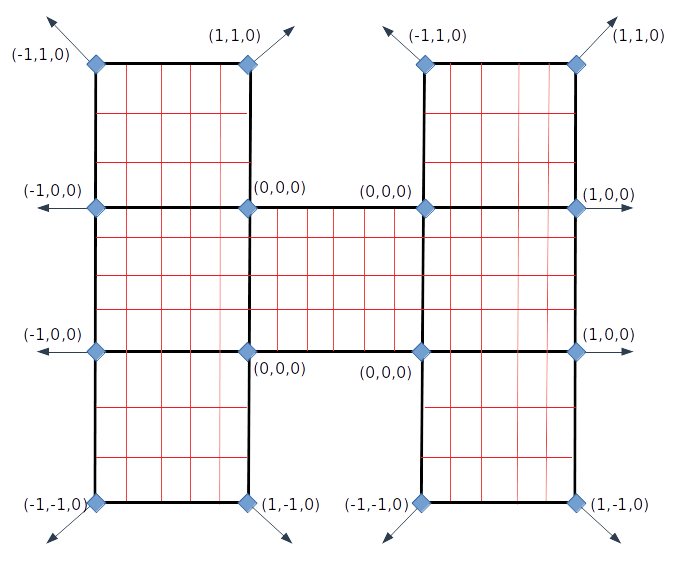
\includegraphics[scale=0.33]{figures/VertBdryNrml.png}
	\caption{Boundary edge normals (left) and boundary vertex normals (right)}
\end{figure}

\subsubsection{Gradient computation on boundaries}
The normal directions stored on each block-boundary entity defines the rule for gradient computation. The normal direction determines the correct one-sided finite difference (FD) scheme to be implemented. (For second-order accurate gradient, fields from two adjacent nodes are required) 

See below, for examples on gradient computation at nodes that falls on boundary block-edge

\begin{figure}[H]
	\centering
	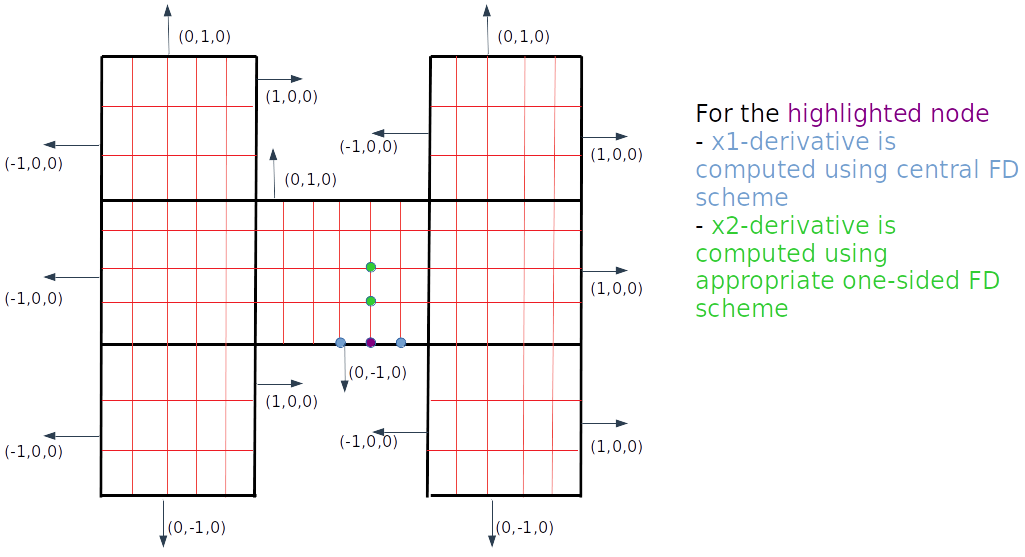
\includegraphics[scale=0.23]{figures/EdgeBdryNrml_Grad1.png}
	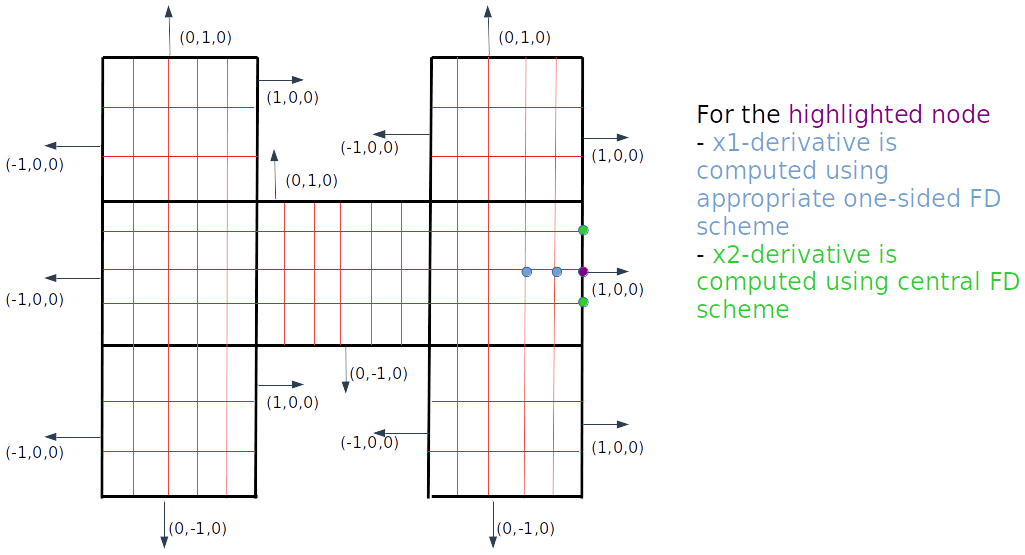
\includegraphics[scale=0.23]{figures/EdgeBdryNrml_Grad2.png}
\end{figure}

See below, for examples on gradient computation at nodes that falls on boundary block-vertices
\begin{figure}[H]
	\centering
	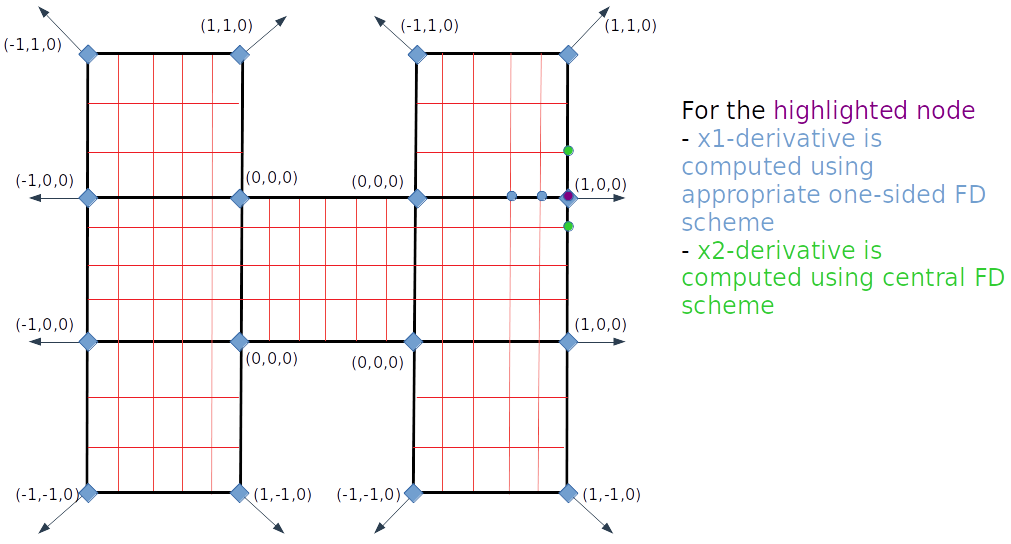
\includegraphics[scale=0.23]{figures/VertBdryNrml_Grad1.png}
	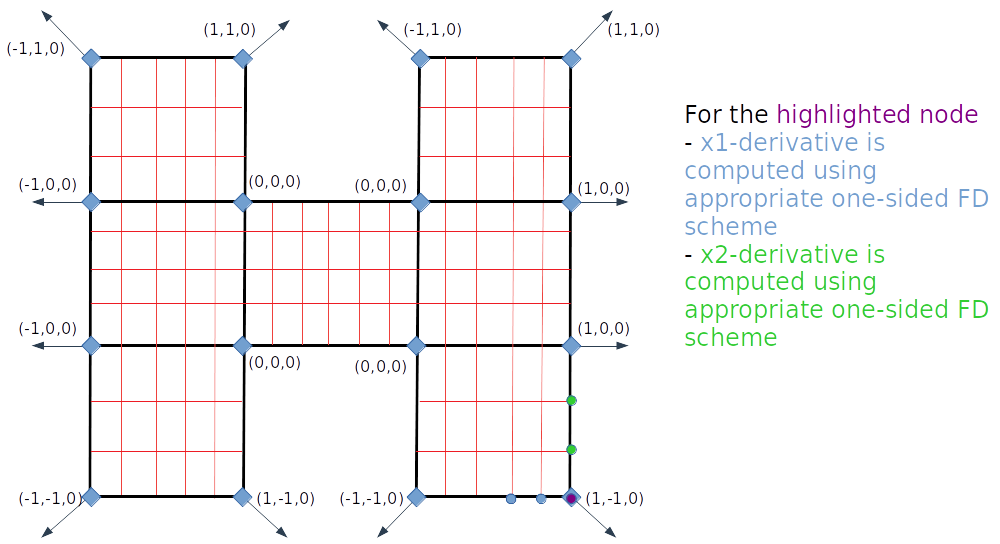
\includegraphics[scale=0.23]{figures/VertBdryNrml_Grad2.png}
	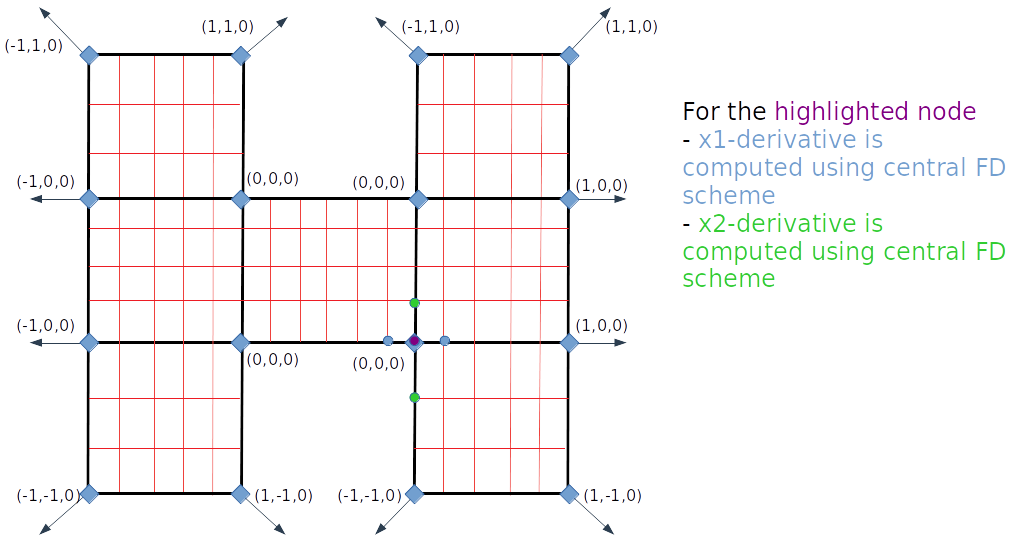
\includegraphics[scale=0.23]{figures/VertBdryNrml_Grad3.png}
\end{figure}
Notice, in the third example, while the node is on boundary it can be treated as a interior node for gradient calculation i.e. central FD scheme can be applied. Hence why the boundary normal for such nodes are set to a zero vector.

\subsubsection{Boundary Element Face IDs}
Boundary faces are defined by the part of a mesh element that touches the boundary of a domain. In 1D, a boundary face is a zero-dimensional entity i.e. point. In 2D, it is a one-dimensional entity i.e. line. 

In \texttt{hpic2}, there are four possible boundary IDs -- east, west, north, south. The boundary element faces are numbered on each boundaries as shown below. First west boundary faces are numbered, then east, then south and finally north faces.  
\begin{figure}[H]
	\centering
	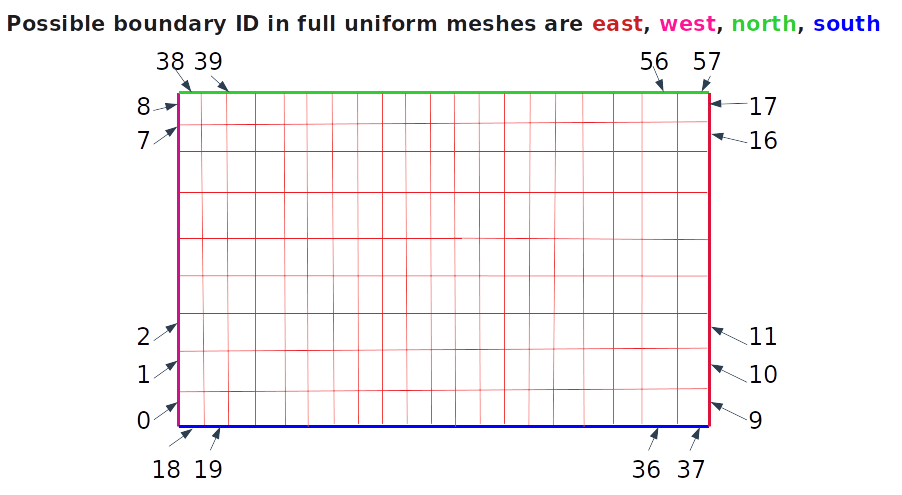
\includegraphics[scale=0.4]{figures/hpic2_bdry_face.png}
\end{figure}

In \texttt{PUMImbbl}, the possible boundary IDs are set of block-edge tags which are classfied as boundary. See example below,
\begin{figure}[H]
	\centering
	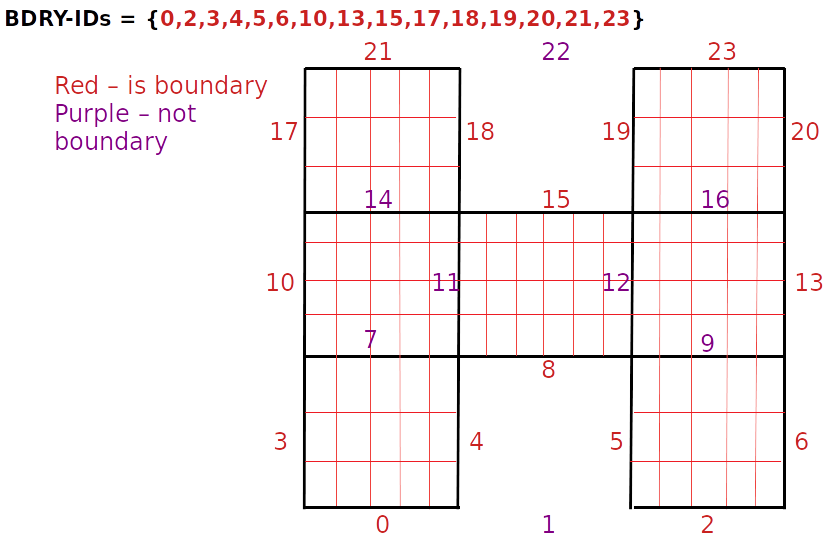
\includegraphics[scale=0.4]{figures/BdryIDs.png}
\end{figure}

In PUMImbbl,
\begin{itemize}
	\item Boundary element faces are numbered on each classified boundary edges
	\item For the example with $BDRY-IDs = \{0,2,3,4,5,6,10,13,15,17,18,19,20,21,23\}$, first element faces in block-edge \#0 are numbered, then block-edge \#2, then \#3 and so on till block-edge \#23
	\item Numbering order inside an block-edge is done towards the positive direction
	\begin{itemize}
		\item For block-edges along x1 – faces are numbered from left to right
		\item For block-edges along x2 – faces are numbered from bottom to top
	\end{itemize}
	\item The starting face ID on each edge is stored, to quickly fetch the face ID of a give a boundary edge ID and an element on that boundary
\end{itemize}
\begin{figure}[H]
	\centering
	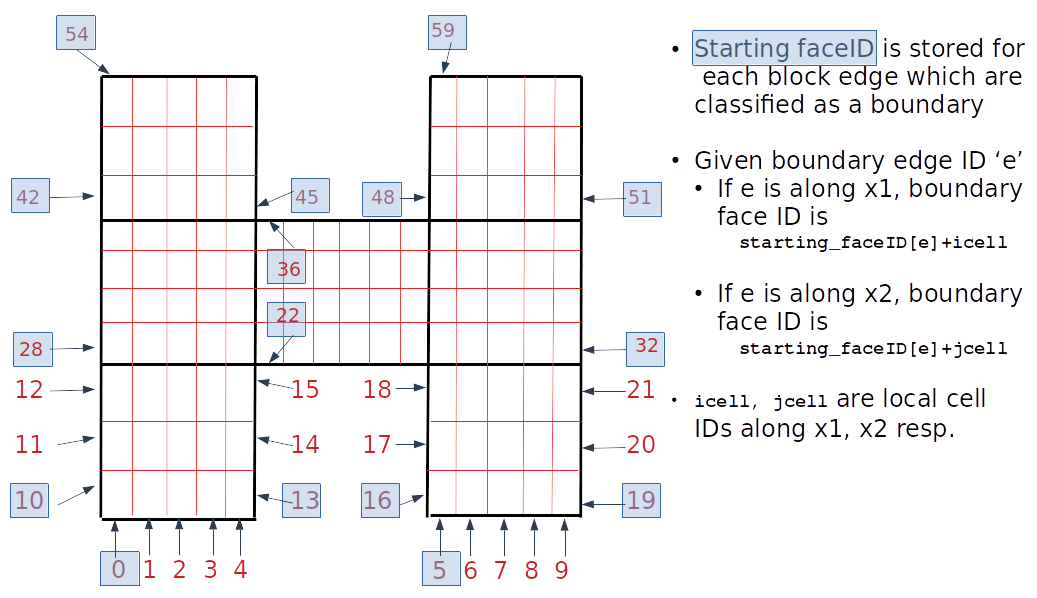
\includegraphics[scale=0.4]{figures/bdry_face_pumi.png}
\end{figure}

\subsection{Node Classification}
The nodes in the PUMImbbl mesh can be classified into three types --
\begin{itemize}
	\item Block-interior nodes -- all nodes that lie completely inside submesh blocks
	\item Block-edge nodes -- all nodes that lie on block edges (excluding the block vertex nodes)
	\item Block-vertex nodes -- all nodes that lie on block vertices
\end{itemize} 

\begin{figure}[H]
	\centering
	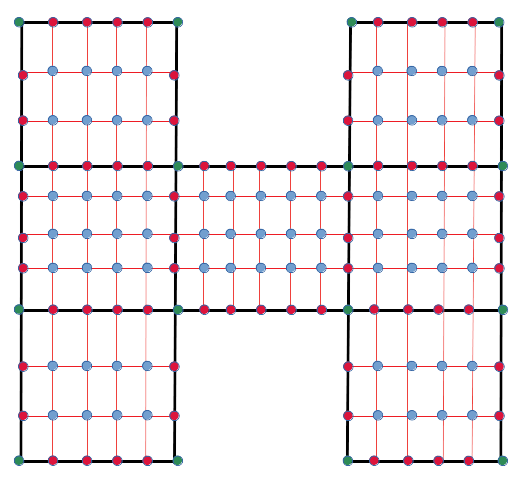
\includegraphics[scale=0.4]{figures/NodeClassification.png}
	\caption{Block interiors nodes are highlighted in blue, Block edge nodes are highlighted in red and Block vertex nodes are highlighted in green}
\end{figure}

This classification comes in handy when operations are to be performed at all mesh nodes. Each type of node will require a different rule to fetch relevant information associated the nodes. When node operations are carried out on GPU device, it is highly inefficient to identify where the given node falls in the domain. In other words, it is highly inefficient to identify the classification type of each node.

\subsubsection{Computing Gradient of Scalar Field}
In the previous subsections we discussed how the gradient can be computed on the boundaries. Here we focus on how to generalize this process for all nodes using node-classification. The idea is to split the loop over all mesh nodes into 3 different loops -- one for each type of nodes. In each loop, first the basic information about the nodes (such as the active submesh-ID to which it belongs to or is adjacent to, the local node IDs etc.,) is obtained. The necessary information for gradient computations such as the global node ID, associated element sizes and directional grading ratio can then be fetched quickly. This saves us from performing highly inefficient global searches which can detrimental to runtime when executed on device. 

\paragraph{Loop over block interior nodes}
Assume all the active block-interior nodes are numbered as shown on the figure below. The numbering starts from the first active block till the last active block (follows the dictionary order inside each block). To recognize the submesh block to which a given block-interior node ID belongs to, we need to store the ID of the last node in each active block. 
\begin{figure}[H]
	\centering
	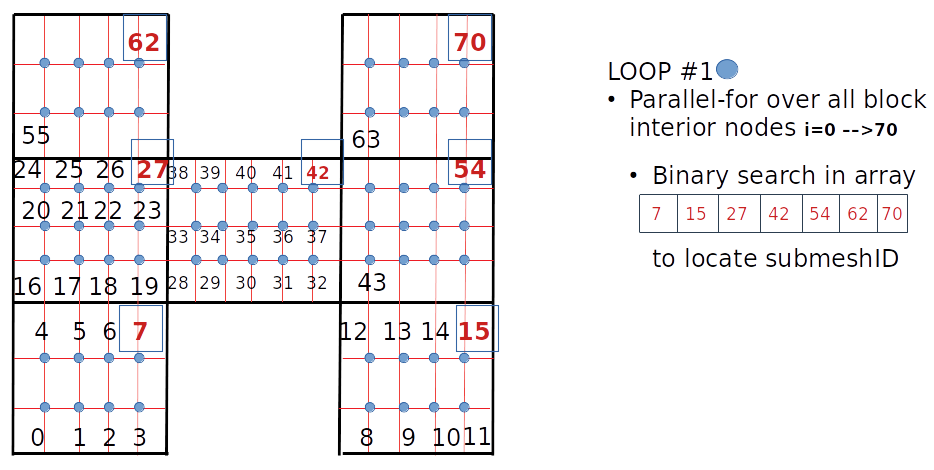
\includegraphics[scale=0.4]{figures/BlockInteriorLoop.png}
\end{figure}

Given a node ID, we first perform a binary search on the list of last nodes to locate the submesh ID of the node (a mapping between i-th active submesh block and actual flattened submesh ID is also explicitly required). Once the flattened submesh ID is known, we can retrieve the directional submesh IDs (\texttt{isub,jsub}) local directional node IDs inside the block (\texttt{inode,jnode}) as well as any local cell IDs (\texttt{icell,jcell}) associated with the node. Properties can then be fetched easily from these IDs.

\paragraph{Loop over block edge nodes}  

Assume all the active block-edge nodes are numbered as shown on the figure below. The numbering starts from the first active edge till the last active edge (follows the positive direction in each edge). To recognize the edge to which a given block-edge node ID belongs to, we need to store the ID of the last node in each active edge. 
\begin{figure}[H]
	\centering
	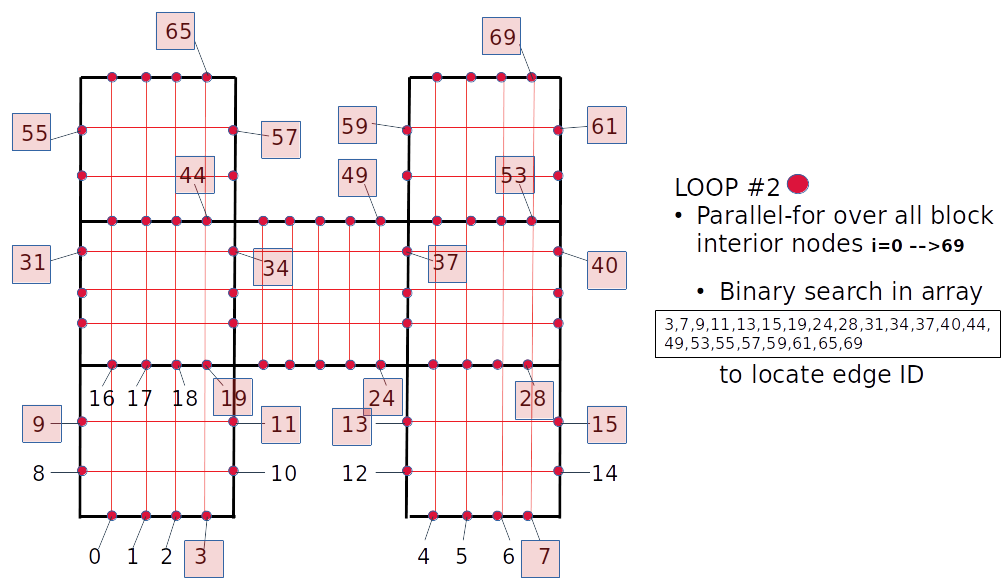
\includegraphics[scale=0.4]{figures/BlockEdgeLoop.png}
\end{figure}

Given a node ID, we first perform a binary search on the list of last nodes to locate the edge ID of the node (a mapping between i-th active edge and actual edge ID is also explicitly required). Once the edge ID is known, we can retrieve the directional submesh IDs (\texttt{isub or jsub}) local directional node IDs inside the edge well as any local cell IDs (\texttt{icell or jcell}) associated with the node. Properties can then be fetched easily from these IDs.

\paragraph{Loop over block vertex nodes}
Since each active vertex is directly mapped to single node, the loop over vertex nodes is equivalent to loop over active block vertices. For ease of access, the properties such as active submesh ID to which give vertex node belongs to, global node ID, etc., are stored in memory.   

%\subsection{2D weight calculations from 1D linear weights}
%\begin{figure}[H]
%	\centering
%	\includegraphics[scale=0.5]{figures/2D-Wgh-calc.png}
%	\caption{(Left) 1D component-wise weight computation\\(Right) 1D component-wise weights to 2D weights}		
%\end{figure}

\section{PUMImbbl Data structure}

\subsection{Submesh-level -- base classes and derived classes}
\begin{lstlisting}
class Submesh{
public:
    double xmin;
    double xmax;
    int Nel;
    double t0;
    double r;
    int Nel_cumulative;
    // enum type 0x01-uniform, 0x02-minBL and 0x04-maxBL
    Meshtype meshtype; 
    Kokkos::View<double*> BL_coords; // BL coords on device
    double *host_BL_coords; // BL coords on host
    Submesh(....):....{}; //Constructor to submesh class
    // Virtual functions on host
    virtual int locate_cell_host(); // using analtyical expressions 
    virtual int update_cell()_host; // using adjacency search
    virtual void calc_weights_host(); // using stored node coordinates
    // Virtual functions not implemented on device
    // device copies of same routines implemented 
    // with switch statements
};
\end{lstlisting}
The submesh class contains block-level mesh parameters. We will have three derived classes, one for each type of meshing.\\

\noindent\textbf{Uniform meshing:}
\begin{lstlisting}
class Uniform_Submesh : public Submesh{
public:
    Uniform_Submesh(....):.....{}; // Constructor to uniform submesh class
    // uniform mesh APIs on host
    int locate_cell_host(); // using analtyical expressions 
    int update_cell_host(); // using adjacency search
    void calc_weights_host();
    .
    .
    .	
    // uniform mesh APIs on device
    KOKKOS_FUNCTION
    int locate_cell();
    KOKKOS_FUNCTION
    int update_cell();
    KOKKOS_FUNCTION
    void calc_weights();
    .
    .
    .
    
};
\end{lstlisting}
\textbf{Left/Bottom BL meshing:}
\begin{lstlisting}
class MinBL_Submesh : public Submesh{
public:
    MinBL_Submesh(....):.....{}; // Constructor to minBL submesh class
    // minBL mesh APIs on host
    void locate_cell_host(); // using analtyical expressions 
    void update_cell_host(); // using adjacency search
    void calc_weights_host();
    .
    .
    .
    // minBL mesh APIs on device
    KOKKOS_FUNCTION
    int locate_cell();
    KOKKOS_FUNCTION
    int update_cell();
    KOKKOS_FUNCTION
    void calc_weights();	
};
\end{lstlisting}
\textbf{Right/Top BL meshing:}
\begin{lstlisting}
class MaxBL_Submesh : public Submesh{
public:
    MaxBL_Submesh(....):.....{}; // Constructor to maxBL submesh class
    // maxBL mesh APIs on host
    void locate_cell_host(); // using analtyical expressions 
    void update_cell_host(); // using adjacency search
    void calc_weights_host();
    .
    .
    .
    // maxBL mesh APIs on device
    KOKKOS_FUNCTION
    int locate_cell();
    KOKKOS_FUNCTION
    int update_cell();
    KOKKOS_FUNCTION
    void calc_weights();
    .
    .
    .	
};
\end{lstlisting}
\textbf{Arbitrary meshing:}
\begin{lstlisting}
class Arbitrary_Submesh : public Submesh{
public:
Arbitrary_Submesh(....):.....{}; // Constructor to maxBL submesh class
// maxBL mesh APIs on host
void locate_cell_host(); // using analtyical expressions 
void update_cell_host(); // using adjacency search
void calc_weights_host();
.
.
.
// Arbitrary mesh APIs on device
KOKKOS_FUNCTION
int locate_cell();
KOKKOS_FUNCTION
int update_cell();
KOKKOS_FUNCTION
void calc_weights();
.
.
.	
};
\end{lstlisting}


\subsection{Mesh-level classes}
\begin{lstlisting}
class MeshOffsets{
// For 2D Mesh with inactive blocks
// Offsets keeps track of nodes/elements in inactive blocks
// Helps speed up computing global element/node ID 
public:
    bool is_fullmesh; // Is mesh with no inactive blocks

    // aux data structure to compute nodeoffset - On device
    Kokkos::View<int**> nodeoffset_start; 
    Kokkos::View<int**> nodeoffset_skip_bot; 
    Kokkos::View<int**> nodeoffset_skip_mid; 
    Kokkos::View<int**> nodeoffset_skip_top;
    // aux data structure to compute element offsets - On device
    Kokkos::View<int**> elemoffset_start; 
    Kokkos::View<int*> elemoffset_skip; 

    // Host copies of aux data structures
    int** host_nodeoffset_start;
    int** host_nodeoffset_skip_bot;
    int** host_nodeoffset_skip_mid;
    int** host_nodeoffset_skip_top;
    int** host_elemoffset_start;
    int* host_elemoffset_skip;

    int Nel_total; // Total active elements in domain
    int Nnp_total; // Total active nodes in domain

    MeshOffsets(){}; // Class constructor
};
\end{lstlisting}

\begin{lstlisting}
class MeshBdry{
// For 2D Mesh with inactive blocks
// Stores block-level boundary edge/vertex information
public:
    // Block edge boundary info
    Kokkos::View<bool*> is_bdry_edge; 
    Kokkos::View<Vector3*> bdry_edge_normal; 
    // Block vertex boundary info
    Kokkos::View<bool*> is_bdry_vert;  
    Kokkos::View<Vector3*> bdry_vert_normal;
    // Starting boundary face ID on each boundary edge 
    Kokkos::View<int*> edge_to_face; 
	
	// Host copies of same info
    bool* host_is_bdry_edge;
    Vector3* host_bdry_edge_normal;
    bool* host_is_bdry_vert;
    Vector3* host_bdry_vert_normal;
    int *host_edge_to_face;

    int Nbdry_faces; // number of boundary element faces

    MeshBdry(){}; // Class constructor

};
\end{lstlisting}

\begin{lstlisting}
class BlockInterface{
    // Class to store informations regarding block interface entities
    public:
    // 1D 
    // Block-interface grading ratio and 
    // component-wise node IDs
    Kokkos::View<double*> if_x1_r; 
    Kokkos::View<int*> if_x1_node; 
    Kokkos::View<double*> if_x2_r; 
    Kokkos::View<int*> if_x2_node; 
    // host-copies of above
    double *host_if_x1_r; 
    int *host_if_x1_node; 
    double *host_if_x2_r; 
    int *host_if_x2_node;
    
    // 2D
    // Vertex Info -- Submesh ID to which
    // it belongs to and global 2D node ID
    Kokkos::View<int*> vert_nodeID; 
    Kokkos::View<int*> vert_subID; 
    // Edge Info -- Submesh ID to which
    // it belongs to and global 2D node ID of 
    // first node on edge
    Kokkos::View<int*> edge_first_nodeID; 
    Kokkos::View<int*> edge_subID; 
    // host-copies of above
    int *host_vert_nodeID; 
    int *host_vert_subID; 
    int *host_edge_first_nodeID; 
    int *host_edge_subID; 
    
    BlockInterface(...){...}; //Class constructor
};
\end{lstlisting}

\begin{lstlisting}
class MeshBST{
    // Data structures necessary to perform
    // binary search to locate block/edge info
    // of classified nodes
    public:
    int total_active_blocks; // total active blocks in domain
    int total_block_nodes; // total active block-interior nodes
    int total_active_edges; // total active edges in domain
    int total_edge_nodes; // total active edge nodes
    // mapping b/w active block to flattened submesh ID
    Kokkos::View<int*> active_blockID; 
    // total active block-interior nodes in all preceding active blocks
    Kokkos::View<int*> block_nodes_cumulative; 
    // total active block elements in all preceding active blocks
    Kokkos::View<int*> block_elems_cumulative; 
    // mapping b/w active edges to actual edge ID
    Kokkos::View<int*> active_edgeID; 
    // total active edge nodes in all preceding active blocks
    Kokkos::View<int*> edge_nodes_cumulative; 
	
    // Host-copies of above
    int* host_active_blockID; 
    int* host_block_nodes_cumulative; 
    int* host_block_elems_cumulative; 
    int* host_active_edgeID; 
    int* host_edge_nodes_cumulative; 
	
	
    MeshBST(..){..}; // Class constructor
};
\end{lstlisting}

\begin{lstlisting}
class Mesh{
public:
    int ndim; // dimension
    int nsubmesh_x1; // number of x1-blocks
    int nsubmesh_x2; // number of x2-blocks
    Kokkos::View<bool**> isactive; // block activity info on device
    bool **host_isactive; // host copy of block activity
    int Nel_total_x1; // number of x1-elements
    int Nel_total_x2; // number of x2-elements
    int Nel_total; // Total mesh elements
    int Nnp_total; // Total mesh nodes
    MeshOffsets offsets; // Object to class MeshOffsets class
    MeshBdry bdry; // Object to class MeshBdry class
    BlockInterface blkif; // Object to class BlockInterface class
    MeshBST bst; // Object to class MeshBST class   
    Mesh(....):...{}; // Class constructor
};
\end{lstlisting}

\subsection{Typedefs for submesh objects}
Memory for submesh are dynamically allocated based on number of blocks. Hence copies are kept on bith device and host.
\begin{lstlisting}
// Submesh object array allocated in GPU using Kokkos View
// cannot be copied to CPU thru Kokkos::deep_copy()
using SubmeshDeviceViewPtr = Kokkos::View<DevicePointer<Submesh>*>;
// Copy of Submesh object array allocated in CPU
using SubmeshHostViewPtr = Submesh*;
// Convenience class for 3D-vectors of double
class Vector3; 
\end{lstlisting}

\subsection{Wrapper struct containing mesh and submesh objects}
\begin{lstlisting}
struct MBBL{
    Mesh mesh; // mesh obj
    SubmeshDeviceViewPtr submesh_x1; // x1-submesh obj in GPU
    SubmeshHostViewPtr host_submesh_x1; // x1-submesh obj in CPU
    SubmeshDeviceViewPtr submesh_x2; // x2-submesh obj in GPU
    SubmeshHostViewPtr host_submesh_x2; // x2-submesh obj in CPU
};
\end{lstlisting}

Object to this structure will be used in \texttt{hpic2} and passed around in mesh APIs

\section{PUMI Mesh initiation}
Mesh initiation is still done through in-memory data structure \texttt{pumi\_inputs}. In hPIC the mesh initiation is performed as

\begin{lstlisting}
// Declare mesh inputs object
pumi::Mesh_Inputs *pumi_inputs;
// allocate memory
pumi_inputs = pumi::inputs_allocate(nsubmesh);
.
.
// parse inputs (from file or commandline) and populate pumi_inputs data structure
.
.	
// Set options for mesh
pumi::Mesh_Options pumi_options;
pumi_options.BL_storage_option = pumi::store_BL_coords_ON;
pumi_options.print_node_option = pumi::print_node_coords_OFF;
pumi_options.print_mesh_connectivity_option = pumi::print_mesh_connectivity_ON;
// Contruct the final pumi wrapper struct
pumi::MBBL pumi_obj = pumi::initialize_MBBL_mesh(pumi_inputs, pumi_options);
// free pumi inputs memory
pumi::inputs_deallocate(pumi_inputs);
\end{lstlisting}

\texttt{MBBL pumi\_obj} variable will ultimately be used in all PUMImbbl mesh APIs as an input as \texttt{pumi::foo(pumi\_obj,...)}



\section{PUMImbbl-APIs -- Get Information (ON HOST)}
\textbf{Mesh-Level Info:}
\begin{table}[H]
	\small
	\begin{tabular}{|l|l|l|l|}
		\hline
		API Name                                & Args                    & \begin{tabular}[c]{@{}l@{}}Return\\ Type\end{tabular} & Description                                      \\ \hline
		\texttt{get\_global\_x1\_min}       & \texttt{MBBL pumi\_obj} & double                                                & Domain lower bound x1-coordinate                \\ \hline
		\texttt{get\_global\_x2\_min}       & \texttt{MBBL pumi\_obj} & double                                                & Domain lower bound x2-coordinate                \\ \hline
		\texttt{get\_global\_x1\_max}       & \texttt{MBBL pumi\_obj} & double                                                & Domain upper bound x1-coordinate                \\ \hline
		\texttt{get\_global\_x2\_max}       & \texttt{MBBL pumi\_obj} & double                                                & Domain upper bound x2-coordinate                \\ \hline
		\texttt{get\_total\_mesh\_elements} & \texttt{MBBL pumi\_obj} & int                                                   & Total active elements in mesh                   \\ \hline
		\texttt{get\_total\_mesh\_nodes}    & \texttt{MBBL pumi\_obj} & int                                                   & Total active nodes in mesh                      \\ \hline
		\texttt{get\_total\_x1\_elements}   & \texttt{MBBL pumi\_obj} & int                                                   & Total elements along x1                         \\ \hline
		\texttt{get\_total\_x2\_elements}   & \texttt{MBBL pumi\_obj} & int                                                   & Total elements along x2                         \\ \hline
		\texttt{get\_mesh\_volume}          & \texttt{MBBL pumi\_obj} & double                                                & Total length in 1D, Active area in 2D of domain \\ \hline
	\end{tabular}
\end{table}
\noindent\textbf{Submesh-Level Info:}
\begin{table}[H]
	\small
	\begin{tabular}{|l|l|l|l|}
		\hline
		API Name                                      & Args                                                                                                      & \begin{tabular}[c]{@{}l@{}}Return \\ Type\end{tabular} & Description                                                                                     \\ \hline
		\texttt{get\_num\_x1\_submesh}                & \texttt{MBBL pumi\_obj}                                                                                   & int                                                    & Number of blocks along x1                                                                       \\ \hline
		\texttt{get\_num\_x2\_submesh}                & \texttt{MBBL pumi\_obj}                                                                                   & int                                                    & Number of blocks along x2                                                                       \\ \hline
		\texttt{get\_total\_submesh\_blocks}          & \texttt{MBBL pumi\_obj}                                                                                   & int                                                    & \begin{tabular}[c]{@{}l@{}}Total mesh blocks in domain\\ including inactive blocks\end{tabular} \\ \hline
		\texttt{get\_num\_x1\_elems\_in\_submesh}     & \begin{tabular}[c]{@{}l@{}}\texttt{MBBL pumi\_obj},\\ \texttt{int isub}\end{tabular}                      & int                                                    & \begin{tabular}[c]{@{}l@{}}Number of elements along x1\\ in given block\end{tabular}            \\ \hline
		\texttt{get\_num\_x2\_elems\_in\_submesh}     & \begin{tabular}[c]{@{}l@{}}\texttt{MBBL pumi\_obj},\\ \texttt{int jsub}\end{tabular}                      & int                                                    & \begin{tabular}[c]{@{}l@{}}Number of elements along x2\\ in given block\end{tabular}            \\ \hline
		\texttt{get\_num\_x1\_elems\_before\_submesh} & \begin{tabular}[c]{@{}l@{}}\texttt{MBBL pumi\_obj},\\ \texttt{int isub}\end{tabular}                      & int                                                    & \begin{tabular}[c]{@{}l@{}}Number of elements along x1\\ in all preceding blocks\end{tabular}   \\ \hline
		\texttt{get\_num\_x2\_elems\_before\_submesh} & \begin{tabular}[c]{@{}l@{}}\texttt{MBBL pumi\_obj},\\ \texttt{int jsub}\end{tabular}                      & int                                                    & \begin{tabular}[c]{@{}l@{}}Number of elements along x2\\ in all preceding blocks\end{tabular}   \\ \hline
		\texttt{get\_total\_elements\_in\_block}      & \begin{tabular}[c]{@{}l@{}}\texttt{MBBL pumi\_obj},\\ \texttt{int isub},\\ \texttt{int jsub}\end{tabular} & int                                                    & \begin{tabular}[c]{@{}l@{}}Total elements in given submesh\\ block\end{tabular}                 \\ \hline
		\texttt{get\_total\_elements\_in\_block}      & \begin{tabular}[c]{@{}l@{}}\texttt{MBBL pumi\_obj},\\ \texttt{int flattened\_sub\_ID}\end{tabular}        & int                                                    & \begin{tabular}[c]{@{}l@{}}Total elements in given submesh\\ block\end{tabular}                 \\ \hline
		\texttt{is\_block\_active\_host}      & \begin{tabular}[c]{@{}l@{}}\texttt{MBBL pumi\_obj},\\ \texttt{int isub},\\ \texttt{int jsub}\end{tabular} & bool                                                    & \begin{tabular}[c]{@{}l@{}}Activity status of given submesh\\ block\end{tabular}                 \\ \hline
		\texttt{is\_block\_active\_host}      & \begin{tabular}[c]{@{}l@{}}\texttt{MBBL pumi\_obj},\\ \texttt{int flattened\_sub\_ID}\end{tabular}        & bool                                                    & \begin{tabular}[c]{@{}l@{}}Activity status of given submesh\\ block\end{tabular}                 \\ \hline
	\end{tabular}
\end{table}
\noindent\textbf{Submesh Vertex related Info:}
\begin{table}[H]
	\small
	\begin{tabular}{|l|l|l|l|}
		\hline
		API Name                                & Args                                                                                   & \begin{tabular}[c]{@{}l@{}}Return\\ Type\end{tabular} & Description                                                                             \\ \hline
		\texttt{get\_total\_mesh\_block\_verts} & \texttt{MBBL pumi\_obj}                                                                & int                                                   & \begin{tabular}[c]{@{}l@{}}Total number of block-vertices\\ in mesh\end{tabular}        \\ \hline
		\texttt{is\_vert\_bdry}                 & \begin{tabular}[c]{@{}l@{}}\texttt{MBBL pumi\_obj},\\ \texttt{int vertID}\end{tabular} & bool                                                  & \begin{tabular}[c]{@{}l@{}}Is given vertex ID part of\\ domain boundary\end{tabular}    \\ \hline
		\texttt{get\_bdry\_vert\_normal}        & \begin{tabular}[c]{@{}l@{}}\texttt{MBBL pumi\_obj},\\ \texttt{int vertID}\end{tabular} & Vector3                                               & \begin{tabular}[c]{@{}l@{}}Boundary normal direction\\ for given vertex ID\end{tabular} \\ \hline
	\end{tabular}
\end{table}
\noindent\textbf{Submesh Edge related Info:}
\begin{table}[H]
	\small
	\begin{tabular}{|l|l|l|l|}
		\hline
		API Name                                       & Args                                                                                                      & \begin{tabular}[c]{@{}l@{}}Return\\ Type\end{tabular} & Description                                                                                           \\ \hline
		\texttt{get\_total\_mesh\_block\_edges}        & \texttt{MBBL pumi\_obj}                                                                                   & int                                                   & \begin{tabular}[c]{@{}l@{}}Total number of block-edges\\ in mesh\end{tabular}                         \\ \hline
		\texttt{is\_edge\_bdry}                        & \begin{tabular}[c]{@{}l@{}}\texttt{MBBL pumi\_obj},\\ \texttt{int edgeID}\end{tabular}                    & bool                                                  & \begin{tabular}[c]{@{}l@{}}Is given edge ID part of\\ domain boundary\end{tabular}                    \\ \hline
		\texttt{get\_bdry\_edge\_normal}               & \begin{tabular}[c]{@{}l@{}}\texttt{MBBL pumi\_obj},\\ \texttt{int edgeID}\end{tabular}                    & Vector3                                               & \begin{tabular}[c]{@{}l@{}}Boundary normal direction\\ for given edge ID\end{tabular}                 \\ \hline
		\texttt{get\_west\_edgeID}                     & \begin{tabular}[c]{@{}l@{}}\texttt{MBBL pumi\_obj},\\ \texttt{int isub},\\ \texttt{int jsub}\end{tabular} & int                                                   & \begin{tabular}[c]{@{}l@{}}edge ID of west edge of \\ given submesh block\end{tabular}                \\ \hline
		\texttt{get\_east\_edgeID}                     & \begin{tabular}[c]{@{}l@{}}\texttt{MBBL pumi\_obj},\\ \texttt{int isub},\\ \texttt{int jsub}\end{tabular} & int                                                   & \begin{tabular}[c]{@{}l@{}}edge ID of east edge of \\ given submesh block\end{tabular}                \\ \hline
		\texttt{get\_south\_edgeID}                    & \begin{tabular}[c]{@{}l@{}}\texttt{MBBL pumi\_obj},\\ \texttt{int isub},\\ \texttt{int jsub}\end{tabular} & int                                                   & \begin{tabular}[c]{@{}l@{}}edge ID of south edge of \\ given submesh block\end{tabular}               \\ \hline
		\texttt{get\_north\_edgeID}                    & \begin{tabular}[c]{@{}l@{}}\texttt{MBBL pumi\_obj},\\ \texttt{int isub},\\ \texttt{int jsub}\end{tabular} & int                                                   & \begin{tabular}[c]{@{}l@{}}edge ID of north edge of \\ given submesh block\end{tabular}               \\ \hline
		\texttt{get\_num\_faces\_on\_edge}             & \begin{tabular}[c]{@{}l@{}}\texttt{MBBL pumi\_obj},\\ \texttt{int edgeID}\end{tabular}                    & int                                                   & \begin{tabular}[c]{@{}l@{}}Number of elements along\\ a given edge ID\end{tabular}                    \\ \hline
		\texttt{get\_starting\_faceID\_on\_bdry\_edge} & \begin{tabular}[c]{@{}l@{}}\texttt{MBBL pumi\_obj},\\ \texttt{int edgeID}\end{tabular}                    & int                                                   & \begin{tabular}[c]{@{}l@{}}Starting boundary element \\ face ID on give boundary \\ edge\end{tabular} \\ \hline
	\end{tabular}
\end{table}
\noindent\textbf{Mesh Element/Node Info}
\begin{table}[H]
	\small
	\begin{tabular}{|l|l|l|l|}
		\hline
		API Name                         & Args                                                                                                                                                                                                                              & \begin{tabular}[c]{@{}l@{}}Return\\ Type\end{tabular} & Description                                                                                                                                                                                                                           \\ \hline
		\texttt{get\_node\_submeshID}    & \begin{tabular}[c]{@{}l@{}}\texttt{MBBL pumi\_obj},\\ \texttt{int knode\_x1},\\ \texttt{int knode\_x2}\end{tabular}                                                                                                               & int                                                   & \begin{tabular}[c]{@{}l@{}}Returns the active \textbf{flattened}\\ \textbf{submesh ID} to which a given\\ node belongs to\end{tabular}                                                                                                \\ \hline
		\texttt{get\_elem\_submeshID}    & \begin{tabular}[c]{@{}l@{}}\texttt{MBBL pumi\_obj},\\ \texttt{int kcell\_x1},\\ \texttt{int kcell\_x2}\end{tabular}                                                                                                               & int                                                   & \begin{tabular}[c]{@{}l@{}}Returns the active \textbf{flattened}\\ \textbf{submesh ID} to which a given\\ element belongs to\end{tabular}                                                                                             \\ \hline
		\texttt{get\_global\_nodeID\_2D} & \begin{tabular}[c]{@{}l@{}}\texttt{MBBL pumi\_obj},\\ \texttt{int knode\_x1},\\ \texttt{int knode\_x2}\end{tabular}                                                                                                               & int                                                   & \begin{tabular}[c]{@{}l@{}}Returns the global node ID (on a 2D\\ mesh) for a given node\end{tabular}                                                                                                                                  \\ \hline
		\texttt{get\_global\_elemID\_2D} & \begin{tabular}[c]{@{}l@{}}\texttt{MBBL pumi\_obj},\\ \texttt{int kcell\_x1},\\ \texttt{int kcell\_x2}\end{tabular}                                                                                                               & int                                                   & \begin{tabular}[c]{@{}l@{}}Returns the global element ID (on a\\ 2D mesh) for a given element\end{tabular}                                                                                                                            \\ \hline
		\texttt{where\_is\_node}         & \begin{tabular}[c]{@{}l@{}}\texttt{MBBL pumi\_obj},\\ \texttt{int knode\_x1},\\ \texttt{int knode\_x2},\\ \texttt{bool *on\_bdry},\\ \texttt{bool *in\_domain},\\ \texttt{int *bdry\_tag},\\ \texttt{int *bdry\_dim}\end{tabular} & void                                                  & \begin{tabular}[c]{@{}l@{}}For given node, tells if \\ - if node is on domain boundary\\ - if node is in active domain\\ - boundary tag (if node is on boundary)\\ - boundary dimension (0=block-vertex,\\ 1=block-edge -- if node is on boundary)\end{tabular} \\ \hline
	\end{tabular}
\end{table}
\noindent\textbf{Directional and flattened IDs}
\begin{table}[H]
	\small
	\begin{tabular}{|l|l|l|l|}
		\hline
		API Name                                                                                                    & Args                                                                                                                                                                                                                              & \begin{tabular}[c]{@{}l@{}}Return\\ Type\end{tabular} & Description                                                                                                                                    \\ \hline
		\begin{tabular}[c]{@{}l@{}}\texttt{flatten\_submeshID\_}\\ \texttt{and\_cellID\_host}\end{tabular}          & \begin{tabular}[c]{@{}l@{}}\texttt{MBBL pumi\_obj},\\ \texttt{int isub},\\ \texttt{int icell},\\ \texttt{int jsub},\\ \texttt{int jcell},\\ \texttt{int *flattened\_subID},\\ \texttt{int *flattened\_cellID}\end{tabular}    & void                                                  & \begin{tabular}[c]{@{}l@{}}Converts the directional\\ submesh and cell IDs to\\ flattened submesh\\ and cell IDs on a 2D\\ mesh\end{tabular}   \\ \hline
		\begin{tabular}[c]{@{}l@{}}\texttt{get\_directional\_submeshID\_}\\ \texttt{and\_cellID\_host}\end{tabular} & \begin{tabular}[c]{@{}l@{}}\texttt{MBBL pumi\_obj},\\ \texttt{int flattened\_subID},\\ \texttt{int flattened\_cellID},\\ \texttt{int *isub},\\ \texttt{int *icell},\\ \texttt{int *jsub},\\ \texttt{int *jcell},\end{tabular} & void                                                  & \begin{tabular}[c]{@{}l@{}}Converts the flattened \\ submesh and cell IDs to \\ directional submesh\\ and cell IDs on a 2D\\ mesh\end{tabular} \\ \hline
	\end{tabular}
\end{table}

\section{PUMImbbl-APIs -- Particle Operations (ON HOST)}
\begin{table}[H]
	\footnotesize
	\begin{tabular}{|l|l|l|l|}
		\hline
		API Name                                      & Args                                                                                                                                                                                                                                      & \begin{tabular}[c]{@{}l@{}}Return\\ Type\end{tabular} & Description                                                                                                                                                                                                                                                             \\ \hline
		\texttt{get\_rand\_point\_in\_mesh\_host}     & \texttt{MBBL pumi\_obj}                                                                                                                                                                                                                   & Vector3                                               & \begin{tabular}[c]{@{}l@{}}Generates a random point\\ coordinate in active region\\ of the domain\end{tabular}                                                                                                                                                          \\ \hline
		\texttt{is\_point\_in\_mesh\_host}            & \begin{tabular}[c]{@{}l@{}}\texttt{MBBL pumi\_obj},\\ \texttt{Vector3 coords}\end{tabular}                                                                                                                                                & bool                                                  & \begin{tabular}[c]{@{}l@{}}Tells if a give point coordinates\\ is in active domain\end{tabular}                                                         \\ \hline
		\texttt{locate\_submesh\_and\_cell\_x1\_host} & \begin{tabular}[c]{@{}l@{}}\texttt{MBBL pumi\_obj},\\ \texttt{double x1\_coord}\\ \texttt{int *isub},\\ \texttt{int *icell}\end{tabular}                                                                                                   & void                                                  & \begin{tabular}[c]{@{}l@{}}Computes a give x1-coordinate's\\ submesh ID and cell ID\\ (along x1-direction)\\ Performs global search\end{tabular}                                                                                                                        \\ \hline
		\texttt{locate\_submesh\_and\_cell\_x2\_host} & \begin{tabular}[c]{@{}l@{}}\texttt{MBBL pumi\_obj},\\ \texttt{double x2\_coord}\\ \texttt{int *jsub},\\ \texttt{int *jcell}\end{tabular}                                                                                                   & void                                                  & \begin{tabular}[c]{@{}l@{}}Computes a give x2-coordinate's\\ submesh ID and cell ID\\ (along x2-direction)\\ Performs global search\end{tabular}                                                                                                                        \\ \hline
		\texttt{calc\_weights\_x1\_host}              & \begin{tabular}[c]{@{}l@{}}\texttt{MBBL pumi\_obj},\\ \texttt{double x1\_coord}\\ \texttt{int isub},\\ \texttt{int icell},\\ \texttt{int *kcell\_x1},\\ \texttt{double *Wgh2\_x1}\end{tabular}                                             & void                                                  & \begin{tabular}[c]{@{}l@{}}Computes linear weight (along\\ x1 direction) for the max-side\\ node as well as component-wise\\ global cell ID (along x1), given \\ x1-coords, submesh ID and \\ cell ID\end{tabular}                                                      \\ \hline
		\texttt{calc\_weights\_x2\_host}              & \begin{tabular}[c]{@{}l@{}}\texttt{MBBL pumi\_obj},\\ \texttt{double x2\_coord}\\ \texttt{int jsub},\\ \texttt{int jcell},\\ \texttt{int *kcell\_x2},\\ \texttt{double *Wgh2\_x2}\end{tabular}                                             & void                                                  & \begin{tabular}[c]{@{}l@{}}Computes linear weight (along\\ x2 direction) for the max-side\\ node as well as component-wise\\ global cell ID (along x2), given \\ x2-coords, submesh ID and \\ cell ID\end{tabular}                                                      \\ \hline
		\texttt{calc\_global\_cellID\_and\_nodeID\_host}    & \begin{tabular}[c]{@{}l@{}}\texttt{MBBL pumi\_obj},\\ \texttt{int isub},\\ \texttt{int jsub},\\ \texttt{int kcell\_x1},\\ \texttt{int kcell\_x2},\\ \texttt{int *global\_cellID},\\ \texttt{int *inp1},\\ \texttt{int *inp3}\end{tabular} & void                                                  & \begin{tabular}[c]{@{}l@{}}Computes global cell and node\\ IDs for a given element\\ (NEEDS the component-wise\\ submesh and cell IDs of the \\ element). Node IDs of bottom-\\ left and top-left nodes of the \\ element are computed. ONLY\\ for 2D mesh\end{tabular} \\ \hline
	\end{tabular}
\end{table}

\section{PUMImbbl APIs -- ON DEVICE}
\noindent\textbf{Submesh-Level Info}
\begin{table}[H]
	\small
	\begin{tabular}{|l|l|l|l|}
		\hline
		API Name                                & Args                    & \begin{tabular}[c]{@{}l@{}}Return\\ Type\end{tabular} & Description                                      \\ \hline
		\texttt{get\_x1\_cellID}       & \begin{tabular}[c]{@{}l@{}}\texttt{MBBL pumi\_obj},\\ \texttt{int isub},\\ \texttt{int icell}\end{tabular} & int                                                & Global cell ID along x1                \\ \hline
		\texttt{get\_x2\_cellID}       & \begin{tabular}[c]{@{}l@{}}\texttt{MBBL pumi\_obj},\\ \texttt{int jsub},\\ \texttt{int jcell}\end{tabular} & int                                                & Global cell ID along x2                \\ \hline
		\texttt{get\_x1\_elem\_size\_in\_submesh}       & \begin{tabular}[c]{@{}l@{}}\texttt{MBBL pumi\_obj},\\ \texttt{int isub},\\ \texttt{int icell}\end{tabular} & double                                                & Element size along x1                \\ \hline
		\texttt{get\_x2\_elem\_size\_in\_submesh}       & \begin{tabular}[c]{@{}l@{}}\texttt{MBBL pumi\_obj},\\ \texttt{int jsub},\\ \texttt{int jcell}\end{tabular} & double                                                & Elemnet size along x2                \\ \hline
	\end{tabular}
\end{table}
\noindent\textbf{Directional and flattened IDs}
\begin{table}[H]
	\small
	\begin{tabular}{|l|l|l|l|}
		\hline
		API Name                                                                                                    & Args                                                                                                                                                                                                                              & \begin{tabular}[c]{@{}l@{}}Return\\ Type\end{tabular} & Description                                                                                                                                    \\ \hline
		\begin{tabular}[c]{@{}l@{}}\texttt{flatten\_submeshID\_}\\ \texttt{and\_cellID}\end{tabular}          & \begin{tabular}[c]{@{}l@{}}\texttt{MBBL pumi\_obj},\\ \texttt{int isub},\\ \texttt{int icell},\\ \texttt{int jsub},\\ \texttt{int jcell},\\ \texttt{int *flattened\_subID},\\ \texttt{int *flattened\_cellID}\end{tabular}    & void                                                  & \begin{tabular}[c]{@{}l@{}}Converts the directional\\ submesh and cell IDs to\\ flattened submesh\\ and cell IDs on a 2D\\ mesh\end{tabular}   \\ \hline
		\begin{tabular}[c]{@{}l@{}}\texttt{get\_directional\_submeshID\_}\\ \texttt{and\_cellID}\end{tabular} & \begin{tabular}[c]{@{}l@{}}\texttt{MBBL pumi\_obj},\\ \texttt{int flattened\_subID},\\ \texttt{int flattened\_cellID},\\ \texttt{int *isub},\\ \texttt{int *icell},\\ \texttt{int *jsub},\\ \texttt{int *jcell},\end{tabular} & void                                                  & \begin{tabular}[c]{@{}l@{}}Converts the flattened \\ submesh and cell IDs to \\ directional submesh\\ and cell IDs on a 2D\\ mesh\end{tabular} \\ \hline
	\end{tabular}
\end{table}
\noindent\textbf{Particle Operations}
\begin{table}[H]
	\footnotesize
	\begin{tabular}{|l|l|l|l|}
		\hline
		API Name                                      & Args                                                                                                                                                                                                                                      & \begin{tabular}[c]{@{}l@{}}Return\\ Type\end{tabular} & Description                                                                                                                                                                                                                                                             \\ \hline
		\texttt{locate\_submesh\_and\_cell\_x1} & \begin{tabular}[c]{@{}l@{}}\texttt{MBBL pumi\_obj},\\ \texttt{double x1\_coord}\\ \texttt{int *isub},\\ \texttt{int *icell}\end{tabular}                                                                                                   & void                                                  & \begin{tabular}[c]{@{}l@{}}Computes a give x1-coordinate's\\ submesh ID and cell ID\\ (along x1-direction)\\ Performs global search\end{tabular}                                                                                                                        \\ \hline
		\texttt{locate\_submesh\_and\_cell\_x2} & \begin{tabular}[c]{@{}l@{}}\texttt{MBBL pumi\_obj},\\ \texttt{double x2\_coord}\\ \texttt{int *jsub},\\ \texttt{int *jcell}\end{tabular}                                                                                                   & void                                                  & \begin{tabular}[c]{@{}l@{}}Computes a give x2-coordinate's\\ submesh ID and cell ID\\ (along x2-direction)\\ Performs global search\end{tabular}                                                                                                                        \\ \hline
		\texttt{update\_submesh\_and\_cell\_x1} & \begin{tabular}[c]{@{}l@{}}\texttt{MBBL pumi\_obj},\\ \texttt{double x1\_coord}\\ \texttt{int isub\_old},\\ \texttt{int icell\_old}, \\\texttt{int *isub},\\ \texttt{int *icell}\end{tabular}                                                                                                   & void                                                  & \begin{tabular}[c]{@{}l@{}}Computes a give x1-coordinate's\\ submesh ID and cell ID\\ (along x1-direction)\\ Performs adjacency search\\ with old IDs\end{tabular}                                                                                                                        \\ \hline
		\texttt{update\_submesh\_and\_cell\_x2} & \begin{tabular}[c]{@{}l@{}}\texttt{MBBL pumi\_obj},\\ \texttt{double x2\_coord}\\ \texttt{int jsub\_old},\\ \texttt{int jcell\_old}, \\ \texttt{int *jsub},\\ \texttt{int *jcell}\end{tabular}                                                                                                   & void                                                  & \begin{tabular}[c]{@{}l@{}}Computes a give x2-coordinate's\\ submesh ID and cell ID\\ (along x2-direction)\\ Performs adjacency search\\ with old IDs\end{tabular}                                                                                                                        \\ \hline
		\texttt{calc\_weights\_x1}              & \begin{tabular}[c]{@{}l@{}}\texttt{MBBL pumi\_obj},\\ \texttt{double x1\_coord}\\ \texttt{int isub},\\ \texttt{int icell},\\ \texttt{int *kcell\_x1},\\ \texttt{double *Wgh2\_x1}\end{tabular}                                             & void                                                  & \begin{tabular}[c]{@{}l@{}}Computes linear weight (along\\ x1 direction) for the max-side\\ node as well as component-wise\\ global cell ID (along x1), given \\ x1-coords, submesh ID and \\ cell ID\end{tabular}                                                      \\ \hline
		\texttt{calc\_weights\_x2}              & \begin{tabular}[c]{@{}l@{}}\texttt{MBBL pumi\_obj},\\ \texttt{double x2\_coord}\\ \texttt{int jsub},\\ \texttt{int jcell},\\ \texttt{int *kcell\_x2},\\ \texttt{double *Wgh2\_x2}\end{tabular}                                             & void                                                  & \begin{tabular}[c]{@{}l@{}}Computes linear weight (along\\ x2 direction) for the max-side\\ node as well as component-wise\\ global cell ID (along x2), given \\ x2-coords, submesh ID and \\ cell ID\end{tabular}                                                      \\ \hline
		\texttt{calc\_global\_cellID\_and\_nodeID}    & \begin{tabular}[c]{@{}l@{}}\texttt{MBBL pumi\_obj},\\ \texttt{int isub},\\ \texttt{int jsub},\\ \texttt{int kcell\_x1},\\ \texttt{int kcell\_x2},\\ \texttt{int *global\_cellID},\\ \texttt{int *inp1},\\ \texttt{int *inp3}\end{tabular} & void                                                  & \begin{tabular}[c]{@{}l@{}}Computes global cell and node\\ IDs for a given element\\ (NEEDS the component-wise\\ submesh and cell IDs of the \\ element). Node IDs of bottom-\\ left and top-left nodes of the \\ element are computed. ONLY\\ for 2D mesh\end{tabular} \\ \hline
		\texttt{push\_particle}    & \begin{tabular}[c]{@{}l@{}}\texttt{MBBL pumi\_obj},\\ \texttt{Vector3 q},\\ \texttt{Vector3 dq}, \\ \texttt{int *isub}, \\ \texttt{int *jsub}, \\ \texttt{int *icell},\\ \texttt{int *jcell}, \\ \texttt{bool *crossed\_bdry},\\ \texttt{int *bdry\_edge\_hit}, \\ \texttt{double *fraction\_done}, \\ \texttt{int *bdry\_faceID\_crossed} \end{tabular} & Vector3                                                  &   \begin{tabular}[c]{@{}l@{}}
			Particle push performed with convex\\ tracking. Input particle coordinate\\vector, displacement vector and IDs.\\ Output info includes\\
			- updated submesh/cell IDs\\
			with adjacency search\\
			- did particle cross boundary\\
			- boundary ID crossed by particle\\
			- fraction of push completed\\
			- boundary face ID crossed 
		\end{tabular} \\ \hline
	\end{tabular}
\end{table}

\section{PUMImbbl APIs -- Input Arguments Explained}
\begin{table}[H]
	\small
	\begin{tabular}{|l|l|l|}
		\hline
		Variable Name                                                                         & Description                                                                                                                   & Valid Inputs                                                                                                           \\ \hline
		\texttt{MBBL pumi\_obj}                                                               & \begin{tabular}[c]{@{}l@{}}Object to MBBL structure used\\ to access all pumi mesh informations,\\ and functions\end{tabular} & \begin{tabular}[c]{@{}l@{}}Valid object has \\ to be initiated from API\\ \texttt{initialize\_MBBL\_mesh}\end{tabular} \\ \hline
		\texttt{int isub}                                                                     & Submesh ID along x1-direction                                                                                                 & int b/w $[1,N_{x_1}]$                                                                                              \\ \hline
		\texttt{int jsub}                                                                     & Submesh ID along x2-direction                                                                                                 & int b/w $[1,N_{x_2}]$                                                                                              \\ \hline
		\begin{tabular}[c]{@{}l@{}}\texttt{int}\\ \texttt{flattened\_subID}\end{tabular}      & \begin{tabular}[c]{@{}l@{}}Componentwise IDs converted i.e.\\ flattened to single ID\end{tabular}                             & int b/w $[0,N_{x_1}N_{x_2}-1]$                                                                                         \\ \hline
		\texttt{int icell}                                                                    & Local x1 cell ID inside a block \texttt{isub}                                                                                 & int b/w $[0,N^{el}_{x_1,\texttt{isub}}-1]$                                                                     \\ \hline
		\texttt{int jcell}                                                                    & Local x2 cell ID inside a block \texttt{jsub}                                                                                 & int b/w $[0,N^{el}_{x_2,\texttt{jsub}}-1]$                                                                     \\ \hline
		\begin{tabular}[c]{@{}l@{}}\texttt{int}\\ \texttt{flattened\_cellID}\end{tabular}     & \begin{tabular}[c]{@{}l@{}}Componentwise IDs converted i.e.\\ flattened to single ID\end{tabular}                             & int b/w $[0,N^{el}_{x_1,\texttt{isub}}N^{el}_{x_2,\texttt{jsub}}-1]$                                           \\ \hline
		\texttt{int vertID}                                                                   & Block-Vertex ID                                                                                                               & int b/w $[0,(N_{x_1}+1)(N_{x_2}+1)-1]$                                                                                 \\ \hline
		\texttt{int edgeID}                                                                   & Block-Edge ID                                                                                                                 & int b/w $[0,2N_{x_1}N_{x_2}+N_{x_1}+N_{x_2}-1]$                                                                                \\ \hline
		\texttt{int kcell\_x1}                                                                & x1-component global cell ID                                                                                                   & int b/w $[0,N^{el,tot}_{x_1}-1]$                                                                               \\ \hline
		\texttt{int kcell\_x2}                                                                & x2-component global cell ID                                                                                                   & int b/w $[0,N^{el,tot}_{x_2}-1]$                                                                               \\ \hline
		\texttt{int knode\_x1}                                                                & x1-component global node ID                                                                                                   & int b/w $[0,N^{el,tot}_{x_1}]$                                                                                 \\ \hline
		\texttt{int knode\_x2}                                                                & x1-component global node ID                                                                                                   & int b/w $[0,N^{el,tot}_{x_2}]$                                                                                 \\ \hline
		\begin{tabular}[c]{@{}l@{}}\texttt{int }\\ \texttt{global\_cell\_ID}\end{tabular}     & \begin{tabular}[c]{@{}l@{}}Global cell ID in 1D, 2D\\ (excluding cells in inactive blocks)\end{tabular}                       & int b/w $0,N^{el,tot}]$                                                                                        \\ \hline
		\texttt{bool on\_bdry}                                                                & \begin{tabular}[c]{@{}l@{}}Tells status of node in 2D mesh\\ if it falls on domain boundary or not\end{tabular}         & 0--true or 1--false                                                                                                    \\ \hline
		\texttt{bool in\_domain}                                                              & \begin{tabular}[c]{@{}l@{}}Tells status of node/coord,\\ if it falls inside domain or not\end{tabular}             & 0--true or 1--false                                                                                                    \\ \hline
		\texttt{int bdry\_tag}                                                                & Edge-ID or Vertex-ID                                                                                                          & Limits based on edge/vertex ID                                                                                         \\ \hline
		\texttt{int bdry\_dim}                                                                & Classification for edge/vertex                                                                                                & 0--vertex and 1--edge                                                                                                  \\ \hline
		\texttt{double Wgh2\_x1}                                                              & \begin{tabular}[c]{@{}l@{}}1D linear-weight along x1\\ corresponding to max-side\end{tabular}                                 & double b/w $[0.0,1.0]$                                                                                             \\ \hline
		\texttt{double Wgh2\_x2}                                                              & \begin{tabular}[c]{@{}l@{}}1D linear-weight along x2\\ corresponding to max-side\end{tabular}                                 & double b/w $[0.0,1.0]$                                                                                             \\ \hline
		\texttt{double x1\_coord}                                                             & x1-coordinate of particle/point                                                                                               & double b/w $[x_1^{min},x_1^{max}]$                                                                                 \\ \hline
		\texttt{double x2\_coord}                                                             & x2-coordinate of particle/point                                                                                               & double b/w $[x_2^{min},x_2^{max}]$                                                                                 \\ \hline
		\begin{tabular}[c]{@{}l@{}}\texttt{int}\\ \texttt{inp1,inp2,inp3,inp4}\end{tabular}   & \begin{tabular}[c]{@{}l@{}}IDs of left-bottom,right-\\ bottom,left-top,right-top node in cell\end{tabular}     & int b/w $[0,N_{np,tot}$                                                                                        \\ \hline
		\texttt{bool crossed\_bdry}                                                           & \begin{tabular}[c]{@{}l@{}}Tells status if particle has crossed a\\ boundary\end{tabular}                                     & 0--true or 1--false                                                                                                    \\ \hline
		\texttt{int bdry\_edge\_hit}                                                          & \begin{tabular}[c]{@{}l@{}}Same as Block-Edge ID where\\ particle crosses boundary\end{tabular}                                        & \begin{tabular}[c]{@{}l@{}}block-edge ID\\classified as boundary\end{tabular}                                                                          \\ \hline
		\begin{tabular}[c]{@{}l@{}}\texttt{double}\\ \texttt{fraction\_done}\end{tabular}     & Fraction of particle push completed                                                                                           & double b/w $[0.0,1.0]$                                                                                             \\ \hline
		\begin{tabular}[c]{@{}l@{}}\texttt{int}\\ \texttt{bdry\_faceID\_crossed}\end{tabular} & \begin{tabular}[c]{@{}l@{}}Boundary Face ID where particle \\crosses a boundary edge\end{tabular}                             & int b/w $[0,N^{bdry-face}-1]$                                                                                  \\ \hline
	\end{tabular}
\end{table}
NOTE: If pointer versions of variable is passed to function argument, it means the API will compute/update the relevant variable during its call.

\section{PUMI-API Usage}
\subsection{Particle-related APIs}
To locate a particle (and compute its partial nodal weight contributions to the 4 nodes) whose coordinates are $(q_1,q_2)$ in 2D, 
\begin{itemize}
	\item [Step-1] Locate the submesh ID and local cell ID (in each direction)
	\item [Step-2] Get the partial component-wise weights corresponding to the max-size node and component-wise global cell IDs (in each direction)
	\item [Step-3] Get the global cell and node IDs in 2D
	\item [Step-4] Compute remaining weights and distribute to the corresponding nodes
\end{itemize}
\begin{verbatim}
int isub, jsub, icell, jcell, kcell_x1, kcell_x2;
int global_2D_cell, left_bottom_node, left_top_node;
double Wgh2_x1, Wgh2_x2, Wgh1_x1, Wgh1_x2;

// Step-1
pumi::locate_submesh_and_cell_x1(pumi_obj, q1, &isub, &icell);
pumi::locate_submesh_and_cell_x2(pumi_obj, q2, &jsub, &jcell);
// After thist step variables isub, jsub will contain component-wise submesh IDs
// and icell, jcell will contain local cell IDs

//Step-2
pumi::calc_weights_x1(pumi_obj, q1, isub, icell, &kcell_x1, &Wgh2_x1);
pumi::calc_weights_x2(pumi_obj, q2, jsub, jcell, &kcell_x2, &Wgh2_x2);
// After thist step variables kcell_x1, kcell_x2 will contain component-wise global
cell IDs and Wgh2_x1, Wgh2_x2 will contain component-wise weights

//Step-3
pumi::calc_global_cellID_and_nodeID(pumi_obj, kcell_x1, kcell_x2, 
&global_2D_cell, &left_bottom_node, &left_top_node);
// After thist step variables global_2D_cell will contain the global element ID and
left_bottom_node, left_top_node will contain the relevant global node IDs 

//Step-4
Wgh1_x1 = 1.0 - Wgh2_x1;
Wgh1_x2 = 1.0 - Wgh2_x2;
int right_bottom_node = left_bottom_node + 1;
int right_top_node = left_top_node + 1;
//distribute to relevant nodes
density[left_bottom_node]  += Wgh1_x1*Wgh1_x2;
density[left_top_node]     += Wgh1_x1*Wgh2_x2;
density[right_bottom_node] += Wgh2_x1*Wgh1_x2;
density[right_top_node]    += Wgh2_x1*Wgh2_x2;

\end{verbatim}

For a pushed particle whose previous submesh and cell IDs are known use the update routines (implements adjacency search with stored BL node coordinates)

\begin{verbatim}
int isub, jsub, icell, jcell, kcell_x1, kcell_x2;
int global_2D_cell, left_bottom_node, left_top_node;
double Wgh2_x1, Wgh2_x2;

// Step-1
pumi::update_submesh_and_cell_x1(pumi_obj, q1, isub, icell, &isub, &icell);
pumi::update_submesh_and_cell_x2(pumi_obj, q2, jsub, jcell, &jsub, &jcell);
// After thist step variables isub, jsub will contain component-wise submesh IDs
// and icell, jcell will contain local cell IDs

//Step-2 to Step-4 remains unchanged
\end{verbatim}

\subsection{Particle Push (with inactive blocks)}
In case of a domain with inactive blocks particle's coordinate update, previously performed as,
\begin{verbatim}
	q1 += dq1;
	q2 += dq2;
	pumi::update_submesh_and_cell_x1(pumi_obj, q1, isub, icell, &isub, &icell);
	pumi::update_submesh_and_cell_x2(pumi_obj, q2, jsub, jcell, &jsub, &jcell);
\end{verbatim}
needs to be replaced with
\begin{verbatim}
	pumi::push_particle(pumi_obj, q1, q2, dq1, dq2, &isub, &jsub, &icell, &jcell, 
	                    &in_domain, &bdry_hit);
\end{verbatim} 
In addition to updating the submesh and cell IDs, we also update the boolean \texttt{in\_domain} to \texttt{false} when a particle goes out of a boundary and the integer \texttt{bdry\_hit} to tag of the edge which the particle crosses to go out of the boundary. For particles inside the domain, \texttt{in\_domain} is set to \texttt{true} and \texttt{bdry\_hit} is set to \texttt{-1}.



\noindent\textbf{NOTE: All the above functions can be called in GPU (i.e. inside \texttt{Kokkos::parallel\_for}). Check \texttt{PUMImbbl\_test.cpp} for an example.}

\subsection{Field-related APIs}
\begin{itemize}
	\item The grading ratio (along a given direction) about an node (from its component-wise global node ID i.e. \texttt{i1, i2}) can be obtained as
	\begin{verbatim}
	// In x1-direction
	double r1 = pumi::return_gradingratio(pumi_obj, pumi::x1_dir, i1);
	
	// In x2-direction
	double r2 = pumi::return_gradingratio(pumi_obj, pumi::x2_dir, i2);
	\end{verbatim}
	
	\item The element-length (along a given direction) for an element (from its component-wise global element/node ID i.e. \texttt{i1, i2}) can be obtained as
	\begin{verbatim}
	// In x1-direction
	double e1 = pumi::return_elemsize(pumi_obj, pumi::x1_dir, kcell_x1,
	pumi::elem_input_offset);
	
	// In x2-direction
	double e2 = pumi::return_elemsize(pumi_obj, pumi::x2_dir, kcell_x2,
	pumi::elem_input_offset);
	\end{verbatim}
	In the above example \texttt{kcell\_x1, kcell\_x2} are element IDs hence the fourth argument is an offset corresponding to element index inputs. If node IDs are to provided as inputs i.e. \texttt{knode\_x1, knode\_x2}, then provide \texttt{pumi::elem\_on\_min\_side\_offset} for element on min-size of node and \texttt{pumi::elem\_on\_max\_side\_offset} for max-side element as last argument
	
	\item The nodal co-volume about a node (from its component-wise global node IDs i.e. \texttt{knode\_x1, knode\_x2}) can be obtained as
	\begin{verbatim}
	// In 1D mesh
	double cv = pumi::return_covolume(pumi_obj, knode_x1);
	// In 2D mesh
	double cv = pumi::return_covolume(pumi_obj, knode_x1, knode_x2);
	\end{verbatim}
	
	\item Information such as active node, boundary node and entity tag/dimension of a boundary node can be obtained by the following function
	\begin{verbatim}
	bool in_domain, on_bdry;
	int bdry_tag, bdry_dim;
	pumi::where_is_node(pumi_obj, knode_x1, knode_x2, 
	                &in_domain, &on_bdry, &bdry_tag, &bdry_dim);
	\end{verbatim}
	After the API call
	\begin{itemize}
		\item If the input node is inside the domain (i.e. not in an inactive block), then \texttt{in\_domain} will be set to \texttt{true}. Otherwise it will be \texttt{false}
		\item If the input node is a boundary node, then \texttt{on\_bdry} will be set to \texttt{true}. Otherwise it will be \texttt{false}
		\item If the input node is a boundary node, then \texttt{bdry\_tag} will be set to the tag of the entity to which the node belongs to. For inactive nodes, the tag will be set to \texttt{-999} and for non-boundary active nodes it will be \texttt{-1}
		\item If the input node is a boundary node, then \texttt{bdry\_dim} will be set to \texttt{0} if it falls on block-vertex and \texttt{1} if it falls on block-edge. For non-boundary and inactive nodes it will be \texttt{-1} 
	\end{itemize}
	 
	
\end{itemize}
\textbf{NOTE: The above APIs can be called only from host. Check \texttt{PUMImbbl\_test.cpp} for an example}


\end{document}
